\chapter{Investigations of the Solar Mean Magnetic Field}\label{chap:SMMF}

%%%%%%%%%%%%%%%%%%%%%%%%%%%%%%%%%%%%%%%%%%%%%%%%%%%%%%%%%%%%%%%%%%%%%
%%%%%%%%%%%%%%%%%%%%%%%%%%%%%%%%%%%%%%%%%%%%%%%%%%%%%%%%%%%%%%%%%%%%%
\section{Introduction}\label{sec:SMMF_intro}

The Sun has a complicated magnetic field structure; many features of the Sun and proxies for the solar activity are related to the evolution of the Sun's magnetic field \citep{wu_solar_2018}.

The solar mean magnetic field (SMMF) is a surprising, non-zero measurement of the imbalance of opposite magnetic flux polarities observed on the full, visible disk of the Sun \citep{svalgaard_suns_1975}, and is defined as the mean line-of-sight (LOS) magnetic field when observing the Sun-as-a-star \citep{scherrer_mean_1977, scherrer_mean_1977-1, garcia_integrated_1999}. In the literature the SMMF is also commonly referred to as the general magnetic field (GMF) \citep{severny_time_1971} or the mean magnetic field (MMF) \citep{kotov_mean_2008} of the Sun.

Observations of the SMMF have typically been made by measuring the Zeeman splitting of spectral lines using a Babcock-type magnetograph \citep{scherrer_mean_1977}, although more recently the SMMF has been calculated from full-disk LOS magnetograms taken from space-borne telescopes such as the Solar Dynamic Observatory Helioseismic and Magnetic Imager (SDO/HMI), in order to understand the morphology of the SMMF \citep{kutsenko_contribution_2017, bose_variability_2018}. It is understood that the strength of the SMMF may vary depending on the spectral line used to measure the SMMF \citep{kotov_mean_2008, kotov_enigmas_2012}, however it is generally accepted in the literature that the SMMF varies slowly with the solar activity cycle, with a amplitude of up to around $\pm 2$ G during solar maximum and $\pm 0.2$ G during solar minimum \citep{plachinda_general_2011}. In addition, the SMMF displays a strong, quasi-coherent rotational signal \citep{chaplin_studies_2003, xie_temporal_2017}, which we assume arises from inhomogeneities on the solar disk with lifetimes of a few rotations.

Despite a wide-ranging existing literature on SMMF observations, spanning several decades, ultimately, our understanding is limited and the SMMF origin remains a crucial, open question in solar physics. The principle component of the SMMF is commonly assumed to be weak, large-scale magnetic flux, distributed over the entire solar disk, rather than active regions (ARs) or sunspots \citep{severny_time_1971, scherrer_mean_1977, xiang_ensemble_2016}. However conversely, \citet{scherrer_mean_1972} found that the SMMF was most highly correlated with only the inner-most one quarter, by area, of the solar disk, which is more sensitive to active latitudes.

In recent literature, \citet{bose_variability_2018} provided an interesting and novel approach to understanding the SMMF whereby they dissected the SMMF by feature identification and pixel-by-pixel analysis of full-disk magnetograms. \citet{bose_variability_2018} concluded that: (i) the observed variability in the SMMF lies in the polarity imbalance of large-scale magnetic field structures on the visible surface of the Sun, (ii) the correlation between the flux from sunspots and the SMMF is statistically insignificant, (iii) and more critically that the background flux dominates the SMMF, accounting for around $89 \%$ of the variation in the SMMF. There still remained a strong component due to rotation in the background magnetic field presented by \citet{bose_variability_2018}, which is indicative of inhomogeneous magnetic features with lifetimes on the order of several solar rotations rather than the shorter-lived, weaker fields usually associated with the large-scale background. 

In order to identify the countours of specific features \citet{bose_variability_2018} used an adaptive thresholding technique on various SDO/AIA images of the solar disc to create binary masks for different types of features. These masks were then applied to scaled SDO/HMI magnetograms in order to segment which features contributed to the SMMF. Upon a closer inspection of the example magnetogram in Figure 2 of the paper, with overplotted contours of identified features, there are clearly regions of strong magnetic flux concentrations in the local vicinity of, and connected to, the identified features that are outside of the contour lines and therefore are allocated to the background magnetic field. It seems an obvious statement to suggest that optical counterparts of the magnetograms will not exactly align with the observed flux in the magnetograms; it should be expected that the magnetic field will manifest itself differently in the optical observations and the magnetograms, which leads one to believe that the background component in this study could mistakenly contain flux from some of the identified features.

In particular, there was a careful treatment of plages in this work from additional chromospheric observations, however a separate handling of faculae in the photosphere was absent from the study, which are well-known to exhibit long lifetimes [CITE ]. Including faculae could have contributed to the completeness of the study. Furthermore, a segmentation of the identified background component into regions of strong and weak field would provide more clarity on the exact morphology of the SMMF, and would have likely provided evidence to conclude whether flux from AR features were incorporated into the background.

Despite these findings, it is known that the strength of the SMMF is weaker during solar minimum, when there are fewer ARs, and stronger during solar maximum, when there are more ARs. This is suggestive that the processes which underpin the evolution of ARs affect the SMMF.

There is another view in the literature which suggests AR flux dominates the SMMF. It was shown earlier by \citet{kutsenko_contribution_2017} that a large component of the SMMF may be explained by strong and intermediate flux regions, that are associated with ARs. Again using a thresholding technique, they showed between $65 \%$ to $95 \%$ of the SMMF could be attributed to strong and intermediate flux, while the fraction of the occupied area varied between $2 \%$ to $6 \%$ of the disk area, depending on the chosen threshold for separating weak and strong flux. This finding suggests that strong, long-lived inhomogeneous regions of magnetic field produce the strong rotation signal in the SMMF. Potential sources could be sunspots, plages, faculae, etc. and \citet{kutsenko_contribution_2017} discuss however that there is an entanglement of strong flux (typically associated with ARs) and intermediate flux (typically associated with network fields and remains of decayed ARs). Disentangling the flux would have provided a more accurate analysis of the SMMF owing to a clearer picture of the main contributor to the SMMF.

The Sun's dynamo and hence magnetic field is directly coupled to the solar rotation. The Sun exhibits latitude-dependent and depth-dependent differential rotation with a sidereal, equatorial period of around 25 days \citep{howe_solar_2009}. To Earth-based observers, the synodic rotation of the Sun is observed at around 27 days, and the SMMF displays a dominant periodicity of around 27 days due to the solar rotation \citep{chaplin_studies_2003, xie_temporal_2017, bose_variability_2018}. It was also reported by \citet{xie_temporal_2017} that the differential solar rotation was observed in the SMMF with measured rotational periods of $28.28 \, \pm \, 0.67$ days and $27.32 \, \pm \, 0.64$ days for the rising and declining phases, respectively, of all of the solar cycles in their considered time-frame.

On the other hand, \citet{xiang_ensemble_2016} utilise ensemble empirical mode decomposition (EEMD) analysis to extract modes of the SMMF and find two rotation periods which are derived from different strengths of magnetic flux elements. They found that a rotation period of 26.6~days was related to a weaker magnetic flux element within the SMMF, while for stronger magnetic flux elements in the SMMF, the measured rotation period is 28.5~days.

Ultimately, to date, our understanding of the SMMF and its origin remains rather limited.




%%%%%%%%%%%%%%%%%%%%%%%%%%%%%%%%%%%%%%%%%%%%%%%%%%%%%%%%%%%%%%%%%%%%%
%%%%%%%%%%%%%%%%%%%%%%%%%%%%%%%%%%%%%%%%%%%%%%%%%%%%%%%%%%%%%%%%%%%%%
\section{Aims}\label{sec:SMMF_aims}

In this work an investigation of high-cadence (sub-minute) observations of the SMMF, made by the Birmingham Solar Oscillations Network (BiSON) \citep{chaplin_bison_1996, chaplin_noise_2005, hale_performance_2016}, was performed. The aim of the investigation was to understand the morphology of the SMMF. 

This work provides a frequency domain analysis of the SMMF data, where a model was built up and fit to the power spectrum of the SMMF which allowed us to understand the characteristics of its possible source(s). 

The rotational modulation signal in the SMMF was clearly observed as several low-frequency peaks in the power spectrum. In addition, the use of the high-cadence data was especially crucial for inferences on components of the SMMF with periods of less than a day at higher frequencies in the power spectrum, with the intention to determine whether the background magnetic field exhibited a stochastically excited component, which evolved on short timescales.

After fitting a model of the power spectrum, artificial data was simulated and comparisons were made to other sources of SMMF data to aid the clarification of the inferences against the observations.



%%%%%%%%%%%%%%%%%%%%%%%%%%%%%%%%%%%%%%%%%%%%%%%%%%%%%%%%%%%%%%%%%%%%%
%%%%%%%%%%%%%%%%%%%%%%%%%%%%%%%%%%%%%%%%%%%%%%%%%%%%%%%%%%%%%%%%%%%%%
\section{Data}\label{sec:SMMF_data}


%%%%%%%%%%%%%%%%%%%%%%%%%%%%%%%%%%%%%%%%%%%%%%%%%%%%%%%%%%%%%%%%%%%%%
\subsection{Summary of the Data Set}

\citet{chaplin_studies_2003} provided the first examination of the SMMF using data from the Birmingham Solar Oscillations Network (BiSON), and the work presented in this paper is a continuation of that study. 

BiSON is a six-station, ground-based, global network of telescopes attempting to continuously monitor the Sun, which principally makes precise measurements of the line-of-sight (LOS) velocity of the photosphere due to solar $p$ mode oscillations. Through the use of polarising optics and additional electronics, the BiSON spectrometers can measure both the disc-averaged LOS velocity and magnetic field in the photosphere \citep{chaplin_studies_2003}, however not all BiSON sites measure the SMMF. 

In this study we focus on the data collected by the Sutherland node, in South Africa, which was also used by \cite{chaplin_studies_2003}. Data are sampled on a 40-second cadence, and the SMMF data collected by the Sutherland station pertains the epochs from 01/1992 -- 12/2012. Over this period, the duty cycle of solar observation is low because of the single-site observations, and averages to be $\sim 15.6\%$ of the total epoch.

A comparison to the SMMF observations made by the Wilcox Solar Observatory (WSO) is given in \citep{chaplin_studies_2003}.

%As a comparison to the BiSON data, SMMF observations were also acquired from the Wilcox Solar Observatory (WSO) (\url{http://wso.stanford.edu/}) \citep{scherrer_mean_1977-1}. The WSO SMMF data are sampled daily from 16/05/1975 -- present day, but for comparison with the BiSON SMMF, we used data over the same temporal range.


%%%%%%%%%%%%%%%%%%%%%%%%%%%%%%%%%%%%%%%%%%%%%%%%%%%%%%%%%%%%%%%%%%%%%
\subsection{Obtaining the SMMF from BiSON}

To acquire the SMMF from BiSON data, the method as described by \citet{chaplin_studies_2003} was adopted; here we discuss the key aspects.

Each  BiSON site employs a resonant scattering spectrometer (RSS) to measure the Doppler shift of the $^{2}\mathrm{S}_{1/2} \, \rightarrow \, ^{2}\mathrm{P}_{1/2}$ line (D1 line) of potassium, at $\sim 770$ nm \citep{brookes_resonant-scattering_1978}. A potassium vapour cell placed within a longitudinal magnetic field Zeeman splits the laboratory line into the two allowed D1 transitions \citep{lund_spatial_2017}. The intensity of the longer wavelength (red; $I_R$) and shorter wavelength (blue; $I_B$) components of the line may be measured by the RSS almost simultaneously, by using polarising optics to switch between the red and blue wings of the line, to form the ratio given by equation~(\ref{eq:ratio}) which is used as a proxy for the Doppler shift from the LOS velocity of the photosphere (see \citet{brookes_observation_1976, brookes_resonant-scattering_1978, elsworth_performance_1995, chaplin_studies_2003, lund_spatial_2017}).  

\begin{equation}
\mathcal{R} = \frac{I_B - I_R}{I_B + I_R}
\label{eq:ratio}
\end{equation}

There are known effects which occur when making observations of the entire solar disk at one time, such as LOS Doppler-imaging and limb-darkening \citep{davies_bison_2014}. Some BiSON stations, that do not measure the SMMF, use optics to spatially scramble incoming sunlight to remove Doppler-imaging effects, to ensure a more accurate measure of the disk-averaged Sun-as-a-star. Sutherland however, is not free from these effects, but they are assumed to be small in the analysis.

Photospheric magnetic fields Zeeman split the Fraunhofer line and the Zeeman-split components have opposite senses of circular polarization \citep{chaplin_studies_2003}. Additional polarising optics are used in the RSS to manipulate the sense of circular polarization (either + or -) that is passed through the instrument. The ratio $\mathcal{R}_{+}$ or $\mathcal{R}_{-}$ is formed, and the ratios $\mathcal{R}_{\pm}$ would be equal if there was no magnetic field present.

The observed ratio ($\mathcal{R}_{\pm}$) may be decomposed as given by equation~(\ref{eq:vel_comp}); where $\mathcal{R}_{\mathrm{orb}}$ is the radial component of the Earth's orbital velocity around the Sun, $\mathcal{R}_{\mathrm{spin}}$ is the component towards the Sun of the Earth's diurnal rotation about its spin axis as a function of latitude and time, $\mathcal{R}_{\mathrm{grs}}$ is from the gravitational red-shift of the solar line due to the Sun's mass \citep{elsworth_techniques_1995, dumbill_observation_1999}. The LOS velocity due to $p$ mode oscillations are given by $\delta {r}_{\mathrm{osc}}(t)$, and $\delta {r}_B(t)$ is due to the magnetic field (+/- from the polarity) \citep{dumbill_observation_1999}. The effect of the magnetic field on the ratio is shown in Fig. \ref{fig:ratio_split}, and it is clear to see from equation~(\ref{eq:R_diff}) that the difference between the opposite magnetic field ratios is twice the magnetic ratio residual.

\begin{equation}
\mathcal{R}_{\pm} = \mathcal{R}_{\mathrm{orb}} + \mathcal{R}_{\mathrm{spin}} + \mathcal{R}_{\mathrm{grs}} + \delta {r}_{\mathrm{osc}}(t) \pm \delta {r}_{\mathrm{B}}(t)
\label{eq:vel_comp}
\end{equation}

\begin{equation}
\mathcal{R}_{+} - \mathcal{R}_{-} = 2 \, \delta {r}_{\mathrm{B}}(t)
\label{eq:R_diff}
\end{equation}

\begin{figure}[ht!]
	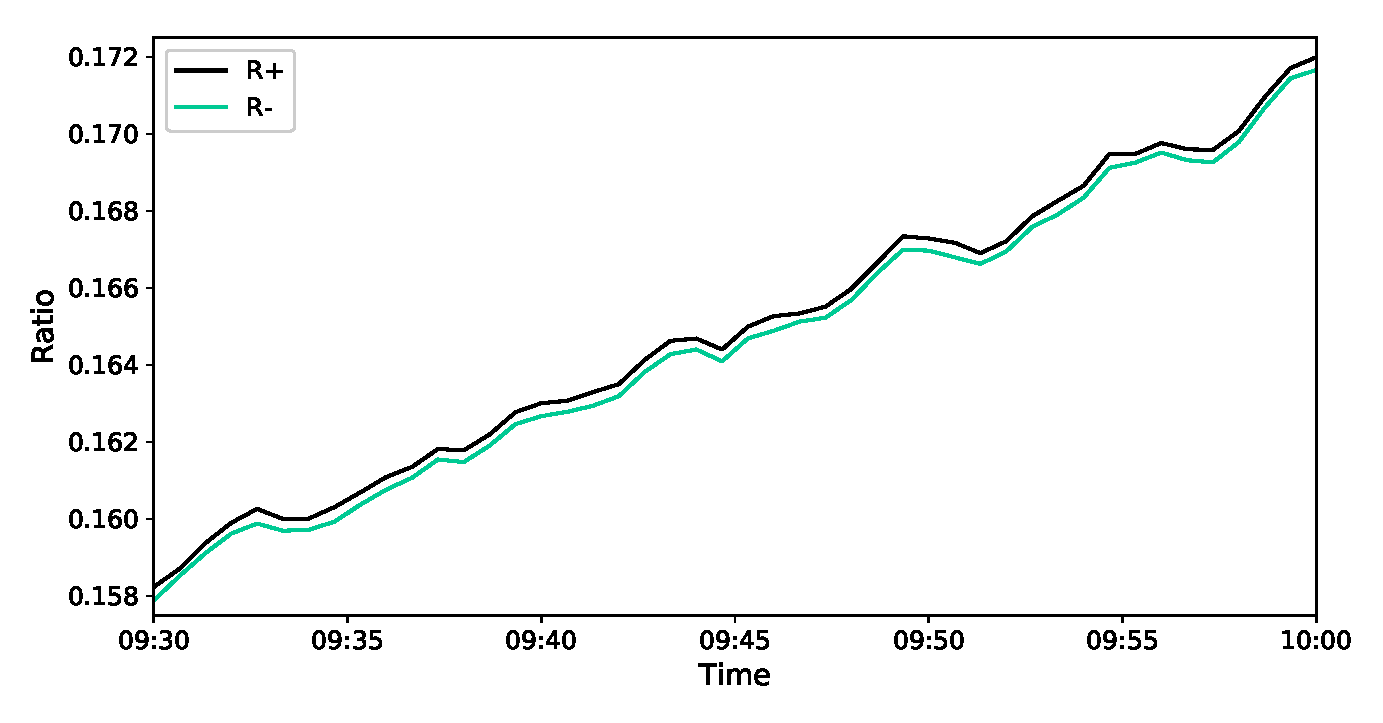
\includegraphics[width=\columnwidth]{Fred_ratio_zoom.eps}
	\caption{An example of the BiSON ratios data over a 30-minute period. The separation between the two ratios is due to the solar mean magnetic field.}
	\label{fig:ratio_split}
\end{figure}

In fact, the BiSON RSS is measuring the velocity variation on the solar disk, and therefore a calibration from the ratio to a velocity is necessary. One method of calibration is achieved by first fitting the observed ratio, averaged over both magnetic polarities, to a 2nd- or 3rd-order polynomial as a function of velocity, as discussed by \citet{elsworth_techniques_1995}. Here we chose to fit the ratio in terms of velocity, $\mathcal{R}_{\mathrm{calc}}(u)$, see equation~(\ref{eq:calc_ratio}):

\begin{equation}
\mathcal{R}_{\mathrm{calc}}(u) = \sum_{n} \mathcal{R}_{n} u^n
\label{eq:calc_ratio}
\end{equation}

where:

\begin{equation}
u = v_{\mathrm{orb}} + v_{\mathrm{spin}}
\label{eq:stn_vel}
\end{equation}

and $v_{\mathrm{orb}}$ is the velocity component related to the ratio,  $\mathcal{R}_{\mathrm{orb}}$; $v_{\mathrm{spin}}$ is related to the ratio, $\mathcal{R}_{\mathrm{spin}}$; and $n$ is the polynomial order.

It is possible to see that through the removal of $\mathcal{R}_{\mathrm{calc}}(u)$ from the observed ratios, one is left with the ratio residuals of the $p$ mode oscillations and the magnetic field (see equation~(\ref{eq:ratio_resid})). Conversion from ratio residuals into velocity residuals uses the calibration given by equation~(\ref{eq:vel_resid}).
%REMOVED: accounting for $\mathcal{R}_{\mathrm{orb}}$, $\mathcal{R}_{\mathrm{spin}}$, and $\mathcal{R}_{\mathrm{grs}}$, 

\begin{equation}
\mathcal{R}_{\pm} - \mathcal{R}_{\mathrm{calc}}(u) = \delta {r}_{\mathrm{osc}}(t) \pm \delta {r}_{\mathrm{B}}(t)
\label{eq:ratio_resid}
\end{equation}

\begin{equation}
\delta v(t) = \left( \frac{d\mathcal{R}_{calc}}{dV} \right)^{-1} \, \delta {r}(t)
\label{eq:vel_resid}
\end{equation}

In order to finally obtain the SMMF in units of magnetic field, one must combine equation~(\ref{eq:R_diff}) and  equation~(\ref{eq:vel_resid}) with the conversion factor in equation~(\ref{eq:K_B}) \citep{dumbill_observation_1999}, where $\mu_B$ is the Bohr magneton, $h$ is Planck's constant, $c$ is the speed of light, and $\nu$ is the frequency of the photons, and the entire procedure can be simplified into equation~(\ref{eq:simplified_SMMF_cal}).

\begin{equation}
K_B = \frac{8}{3} \, \frac{\mu_B}{h} \, \frac{c}{\nu} \approx 2.89... \, \mathrm{ms}^{-1} \, \mathrm{G}^{-1}
\label{eq:K_B}
\end{equation}

\begin{equation}
B(t) = \frac{1}{2} \left( \frac{d\mathcal{R}_{calc}}{dV} \right)^{-1} (\mathcal{R}_{+} - \mathcal{R}_{-}) / K_B
\label{eq:simplified_SMMF_cal}
\end{equation}

Through the application of this methodology, one acquires the SMMF as shown in Fig.~(\ref{fig:SMMF_TS}). The power spectrum of the SMMF is shown in Fig.~(\ref{fig:SMMF_FT}), and it shows a strong rotational signal at a period of $\sim27$~days. 
%The power spectrum of the SMMF is shown again in Fig.~\ref{fig:SMMF_40s_PSD} on a logarithmic scale covering the entire frequency range, which highlights the broadband background component of the power spectrum. As the data we are working with has a low fill, this manifests itself with certain repeated structures in the power spectrum; however if there is a weak, stochastic, ephemeral background component in the SMMF, we shall measure it in this component.


\begin{figure}[ht!]
	\centering
	\subfloat[BiSON SMMF 40-second cadence time series \label{fig:SMMF_TS}]{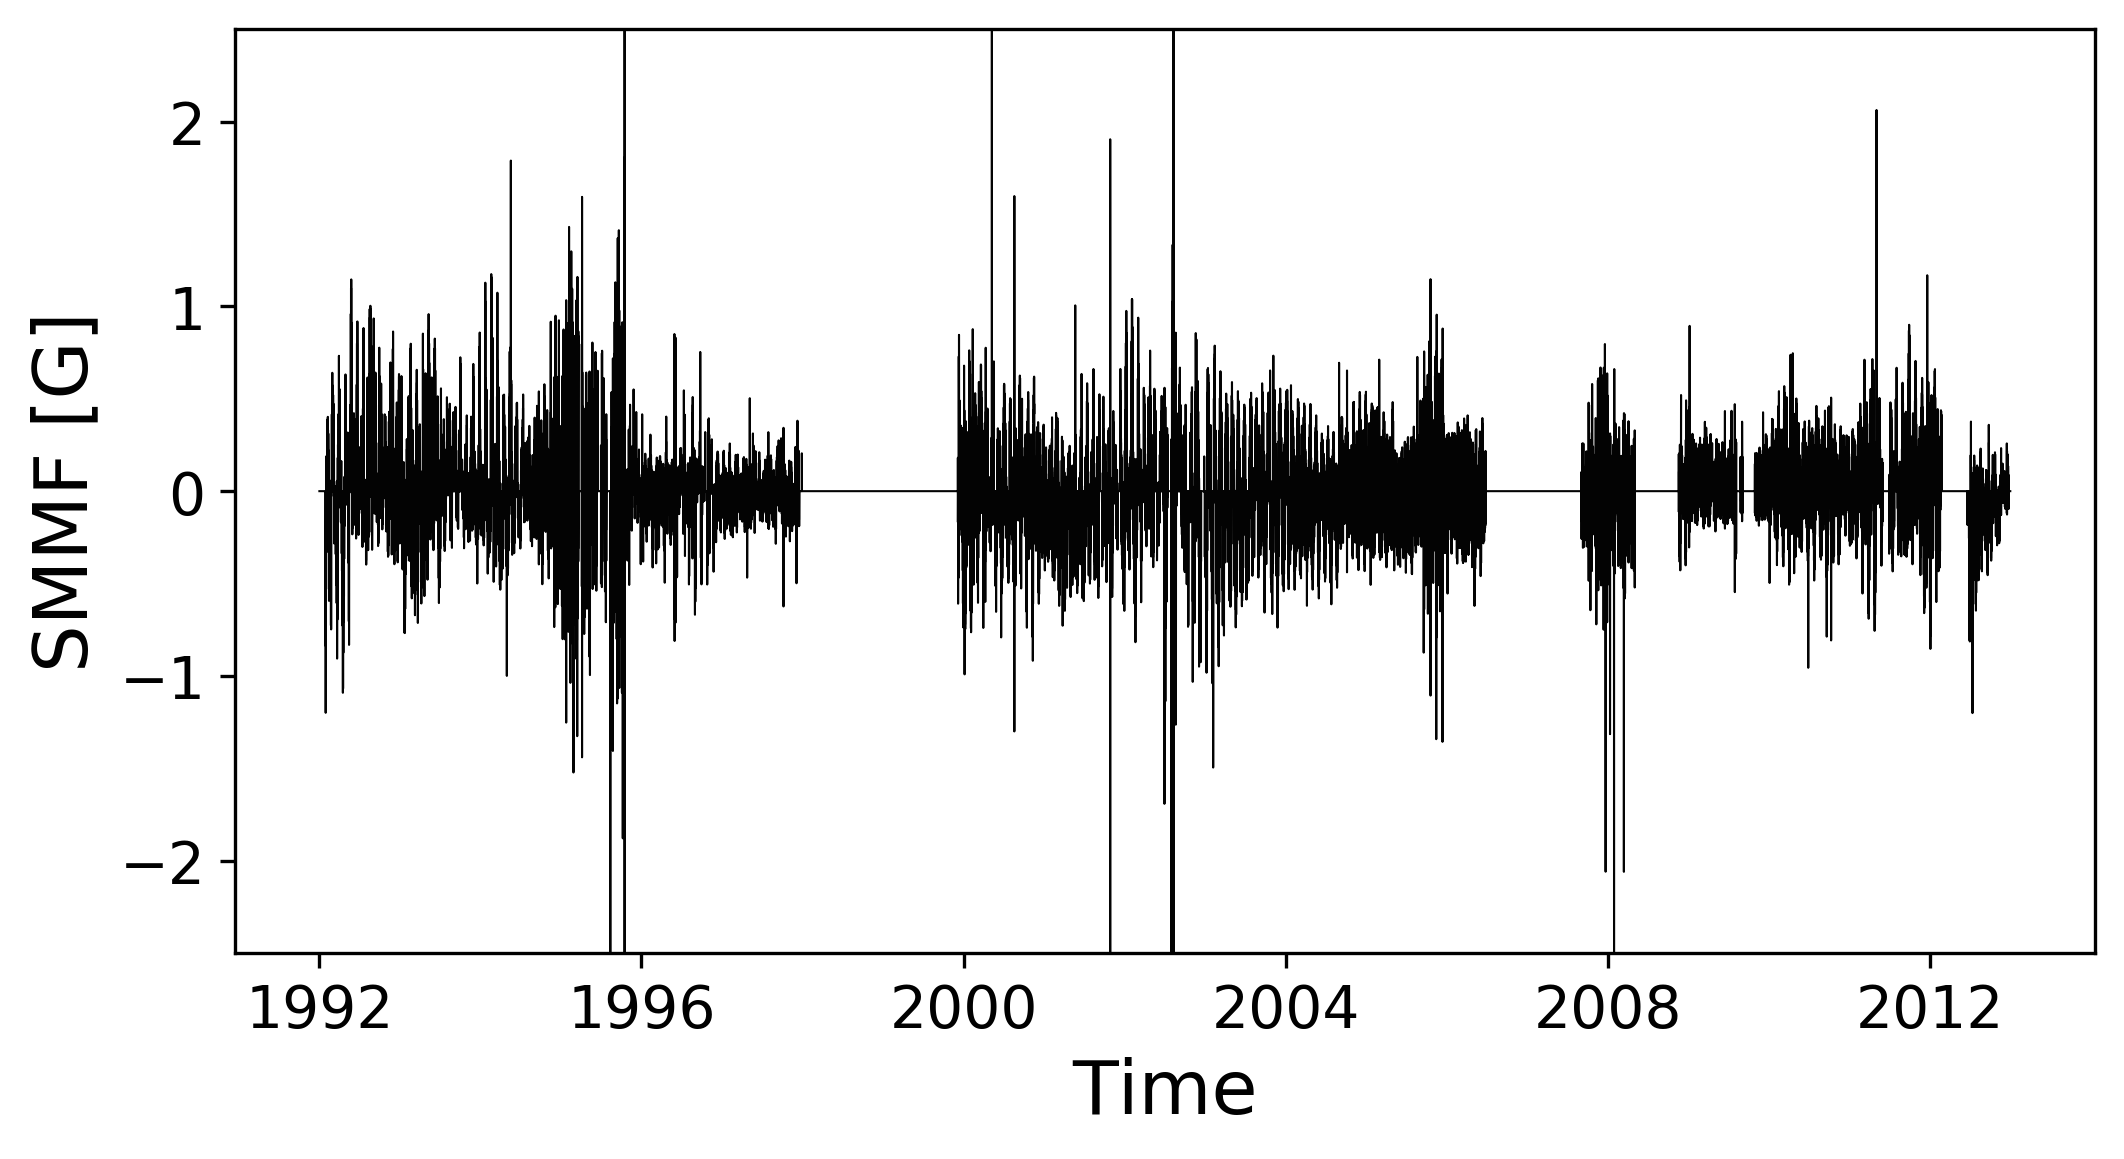
\includegraphics[width=0.98\columnwidth]{BiSON_full_TS.png}} \\ 
	\centering
	\subfloat[Power spectral density of the BiSON SMMF \label{fig:SMMF_FT}]{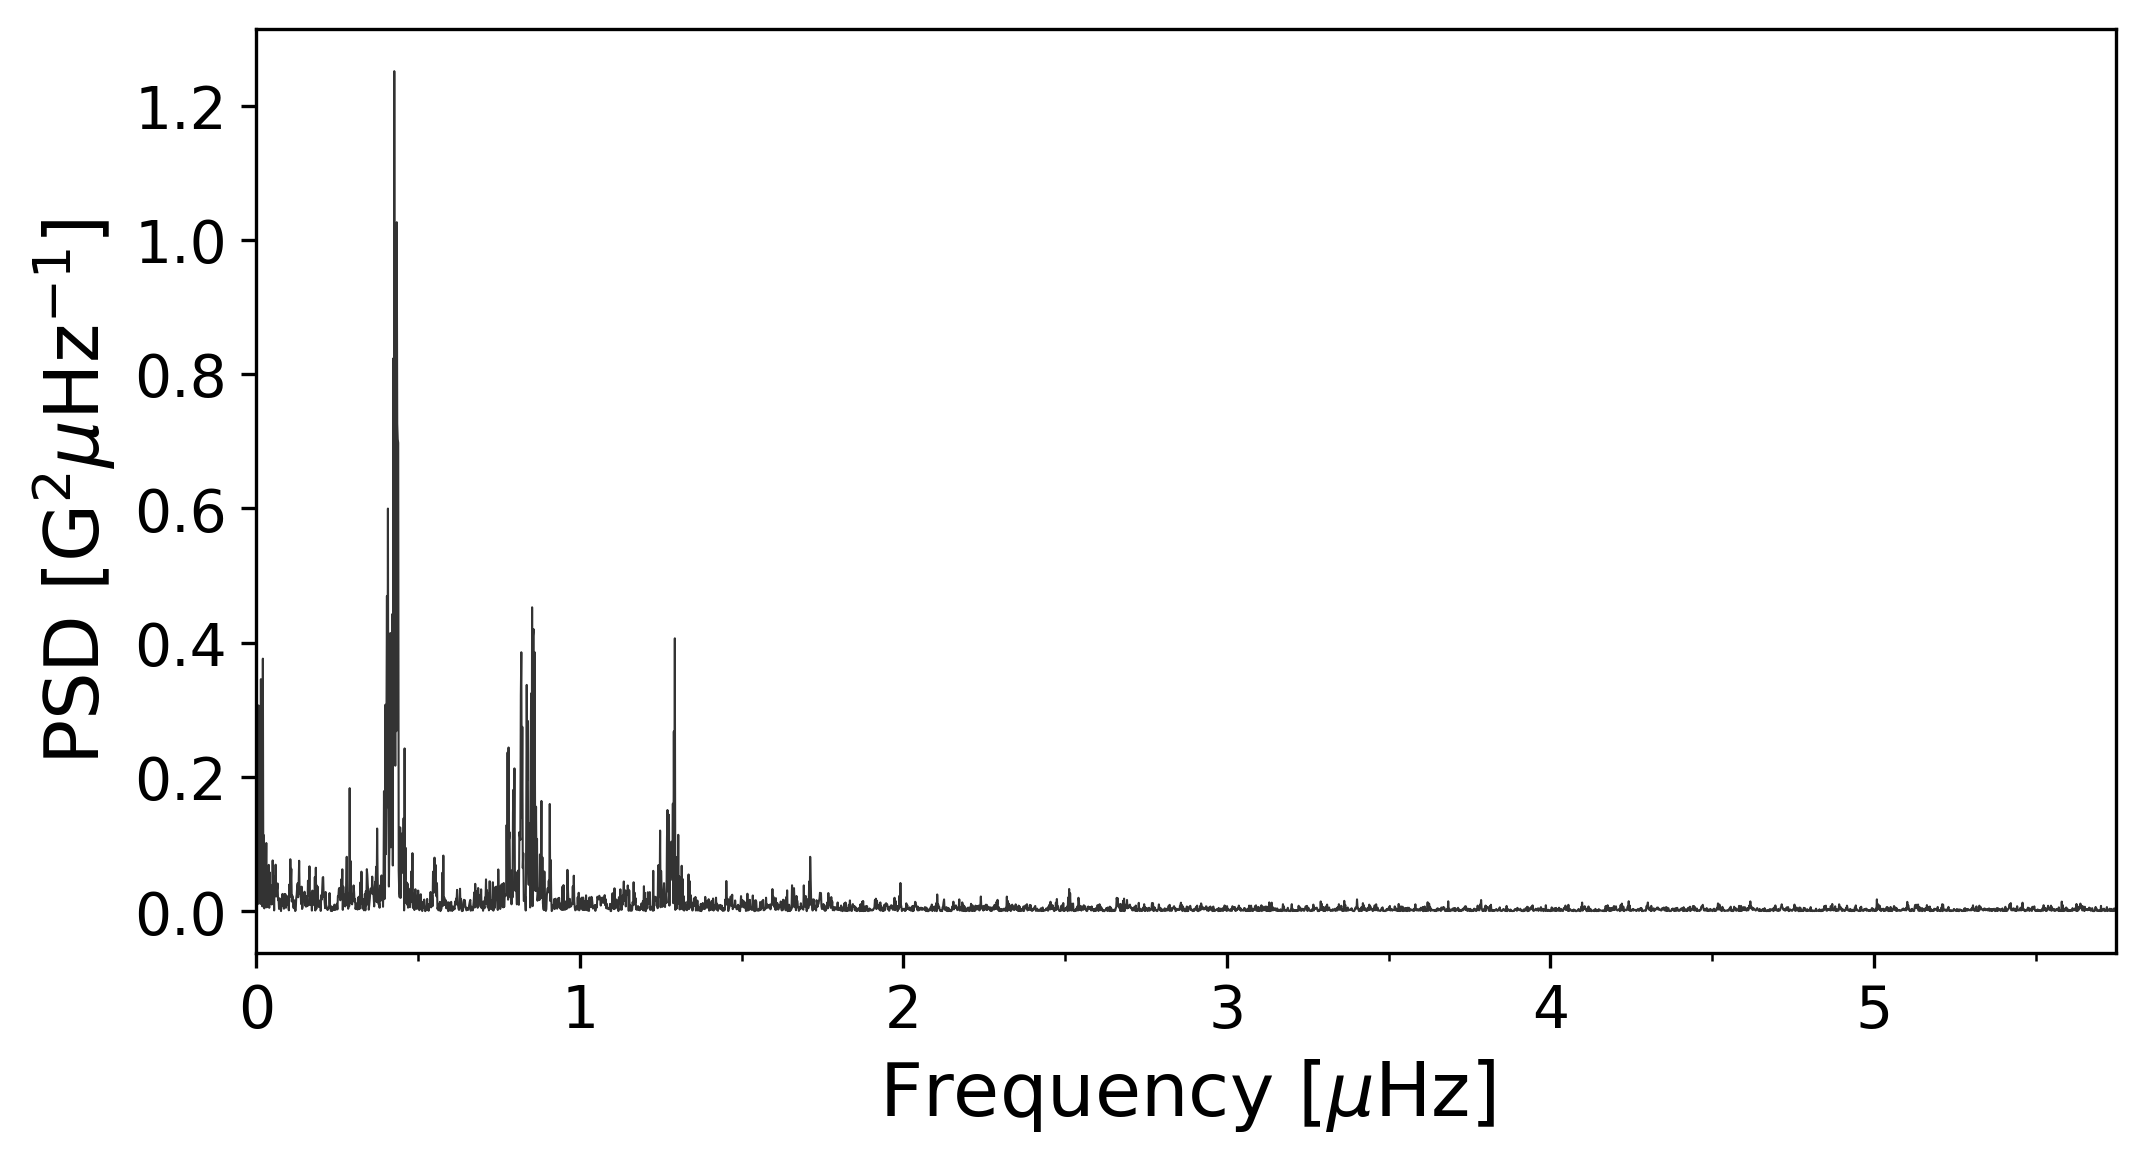
\includegraphics[width=\columnwidth]{BiSON_lin_mu_PSD.png}}
	\caption{(a) 40-second cadence observations of the SMMF from the Sutherland BiSON station between 1992 and 2012. The sense of the field was chosen to match the \citet{chaplin_studies_2003} and the WSO observations, where positive is for a field pointing outwards from the Sun. (b) Power spectrum of the SMMF on a 40-second cadence truncated to $10 \mu\mathrm{Hz}$, however the nyquist frequency is 12.5 mHz.}  
	\label{fig:BiSON_SMMF}
\end{figure}


%%%%%%%%%%%%%%%%%%%%%%%%%%%%%%%%%%%%%%%%%%%%%%%%%%%%%%%%%%%%%%%%%%%%%
\subsection{Comparison between WSO and BiSON}

The relationship between the SMMF measured by the Sutherland BiSON station and the SMMF measured by the Stanford WSO was examined. The daily SMMF measured by the Stanford WSO and Sutherland BiSON station are plotted in Fig~\ref{fig:BiSON_and_WSO}.

\begin{figure}[ht!]
    \centering
	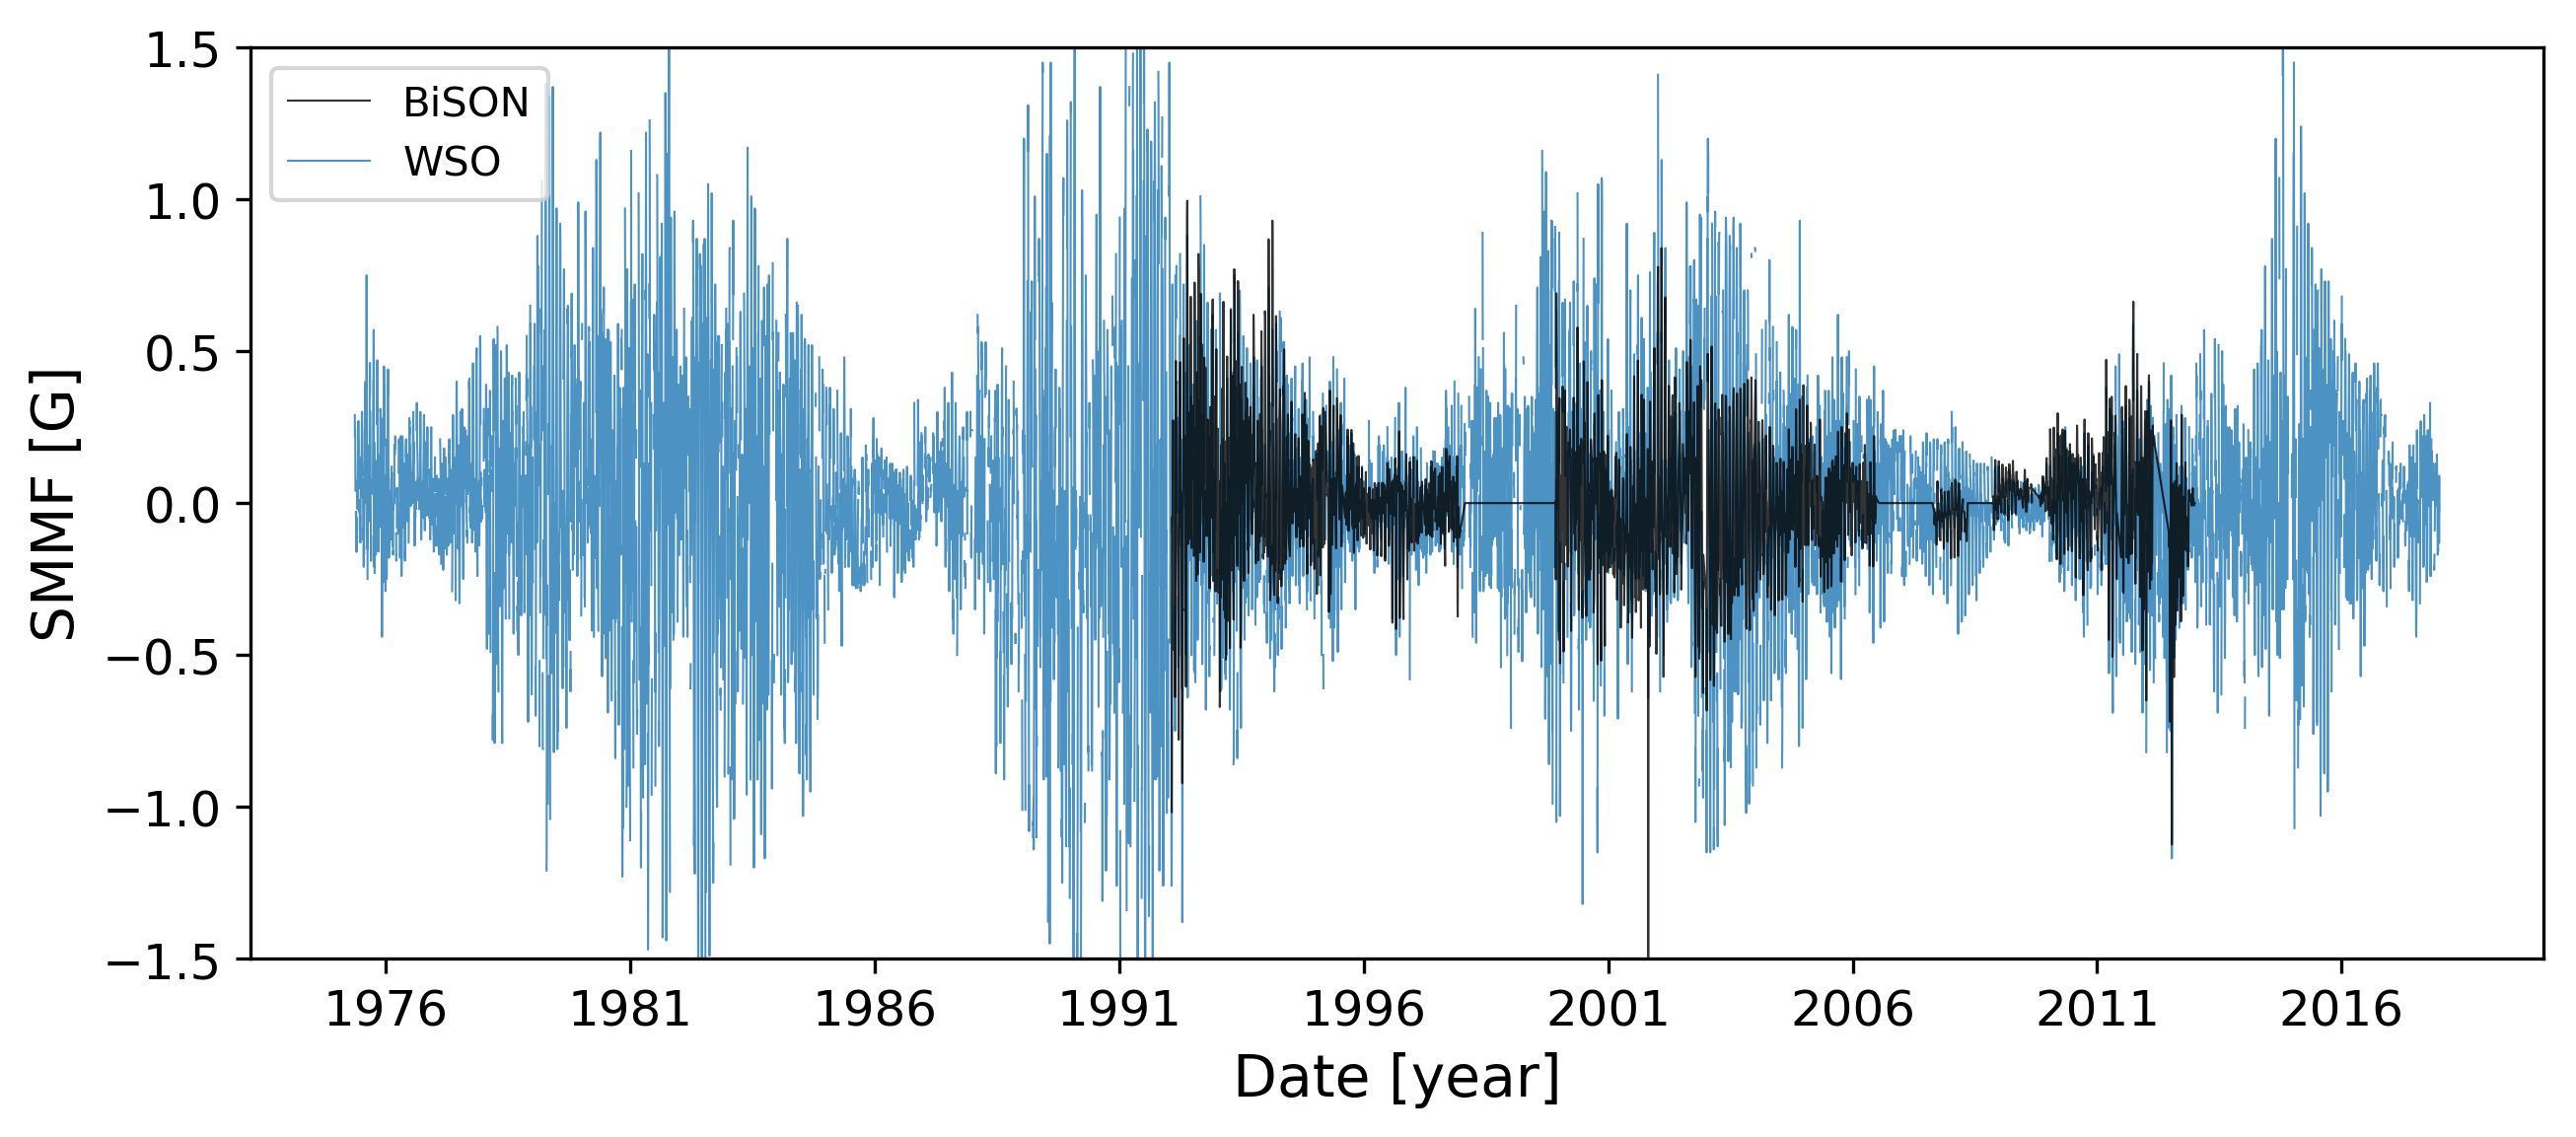
\includegraphics[width=\columnwidth]{BiSON_and_WSO.png}
    \caption{Daily averaged SMMF measured by WSO (blue) and by the Sutherland BiSON station (black).}
    \label{fig:BiSON_and_WSO}
\end{figure}

Fig.~\ref{fig:BiSON_vs_WSO} shows the correlation between the two data sets. The gradient of the line is $0.4999\pm0.0001$ and informs us that the BiSON SMMF is half of the magnitude of that observed by WSO. This discrepancy may be due to the measurements of the SMMF using different spectral lines, hence their levels of formation in the solar atmosphere, and the divergence of magnetic field lines with altitude; an altitude difference of 100--200 km could lead to a difference of 30--50$\%$.

\begin{figure}[ht!]
    \centering
	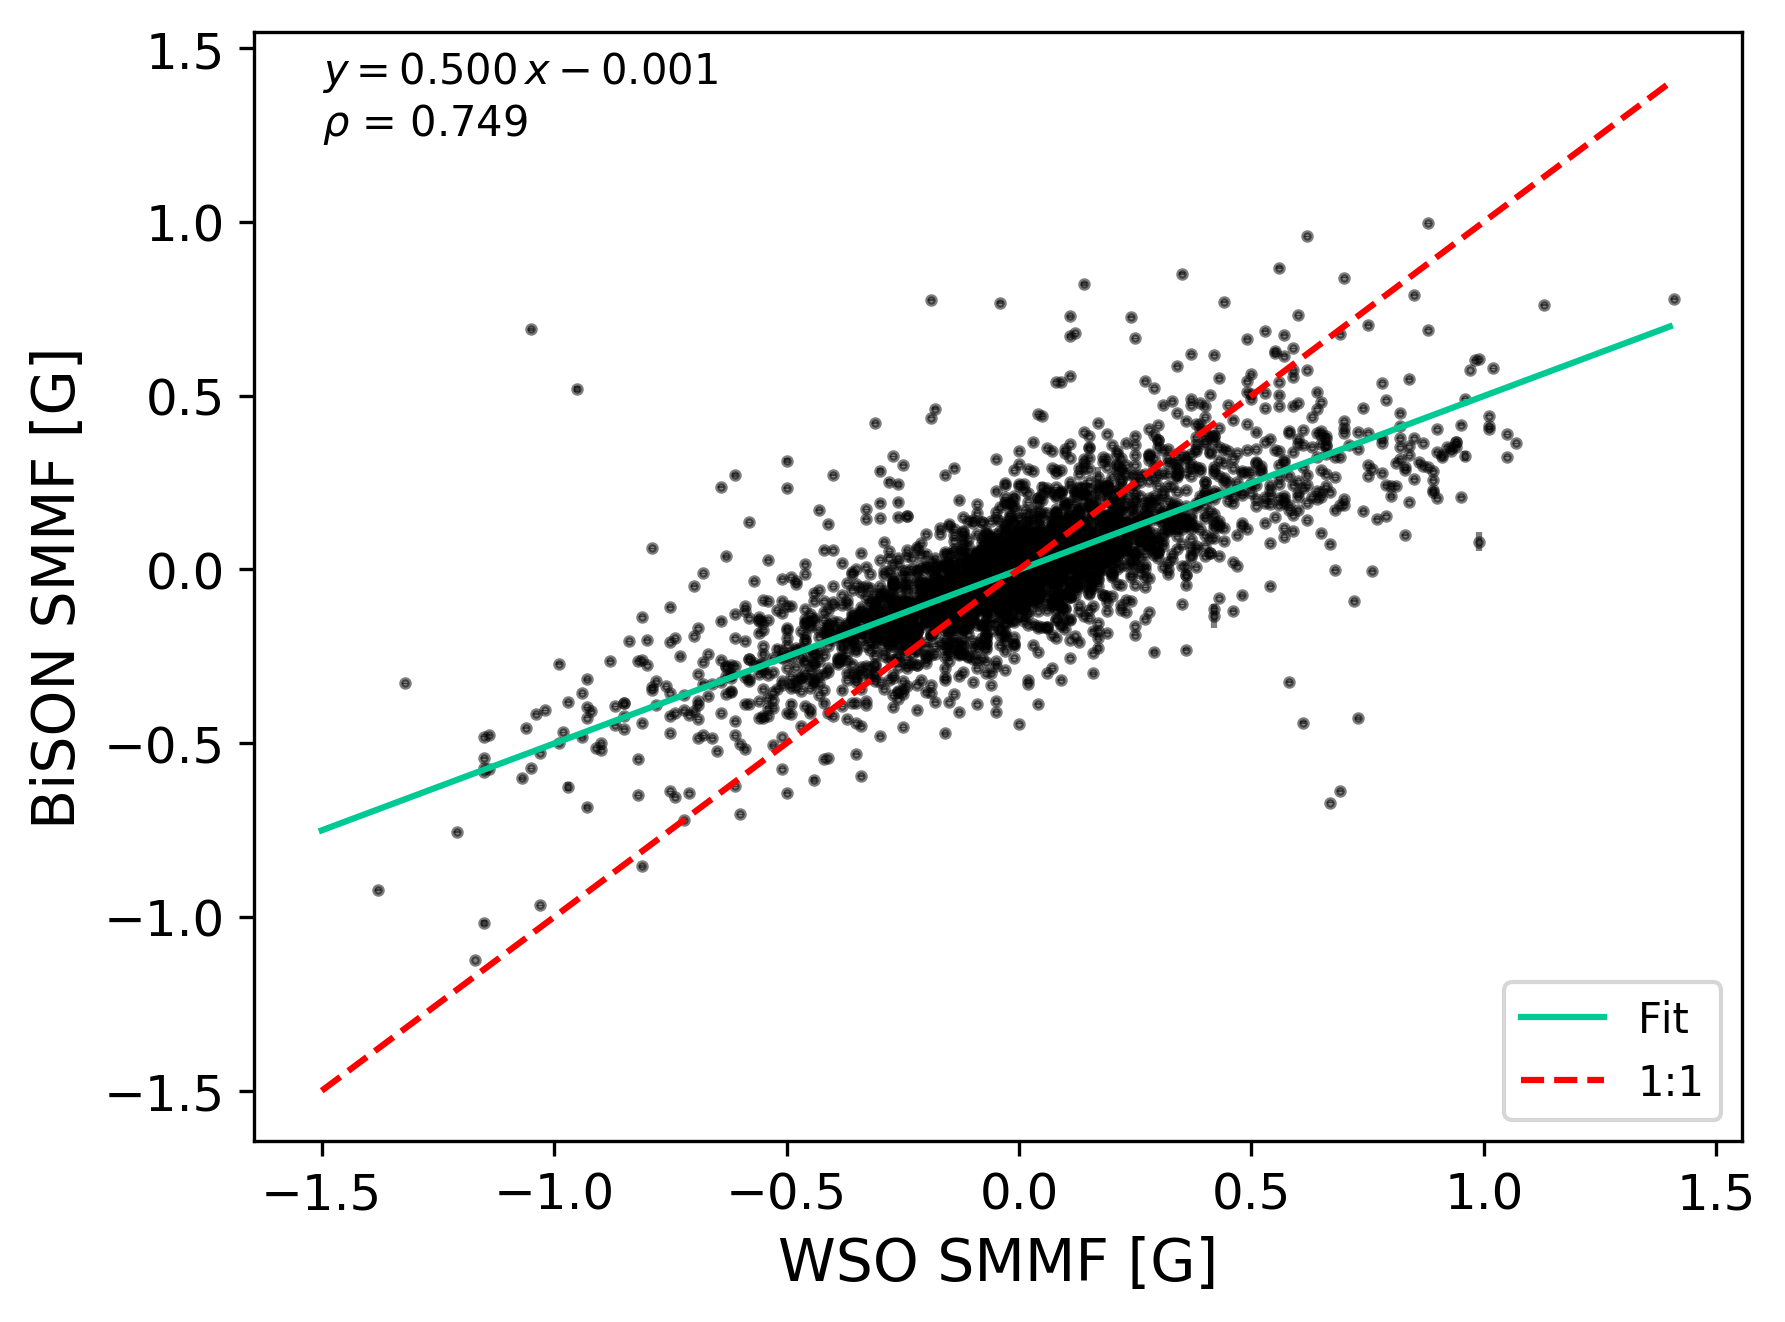
\includegraphics[width=0.75\columnwidth]{BiSON_vs_WSO.png}
    \caption{Correlation between the daily SMMF measured by WSO and by the Sutherland BiSON station. The green line provides the fit to the data, while the red line shows a 1:1 relation for comparison.}
    \label{fig:BiSON_vs_WSO}
\end{figure}

%Interestingly \citet{chaplin_studies_2003} stated that the SMMF observed by the Sutherland BiSON station was roughly twice that of WSO... [not sure how to handle this...?]

%This suggests that there is a factor of 4 difference between the measurements of the SMMF by \citet{chaplin_studies_2003} and in this work. A factor of 2 could be explained due to the factor of a half that is necessary in equation~\ref{eq:B(t)}, but a factor of 4 is not understood. 



%%%%%%%%%%%%%%%%%%%%%%%%%%%%%%%%%%%%%%%%%%%%%%%%%%%%%%%%%%%%%%%%%%%%%
%%%%%%%%%%%%%%%%%%%%%%%%%%%%%%%%%%%%%%%%%%%%%%%%%%%%%%%%%%%%%%%%%%%%%
\section{Methodology}\label{sec:SMMF_method}


%%%%%%%%%%%%%%%%%%%%%%%%%%%%%%%%%%%%%%%%%%%%%%%%%%%%%%%%%%%%%%%%%%%%%
\subsection{Identifying Features in the SMMF Power Spectrum}

The full power spectrum of the 40-second cadence SMMF is shown in Figure~\ref{fig:BiSON_FT_full}, covering a frequency range up to the Nyquist frequency of 12500 mHz, with a resolution of 1.516 nHz. 

\begin{figure}[ht!]
	\centering
	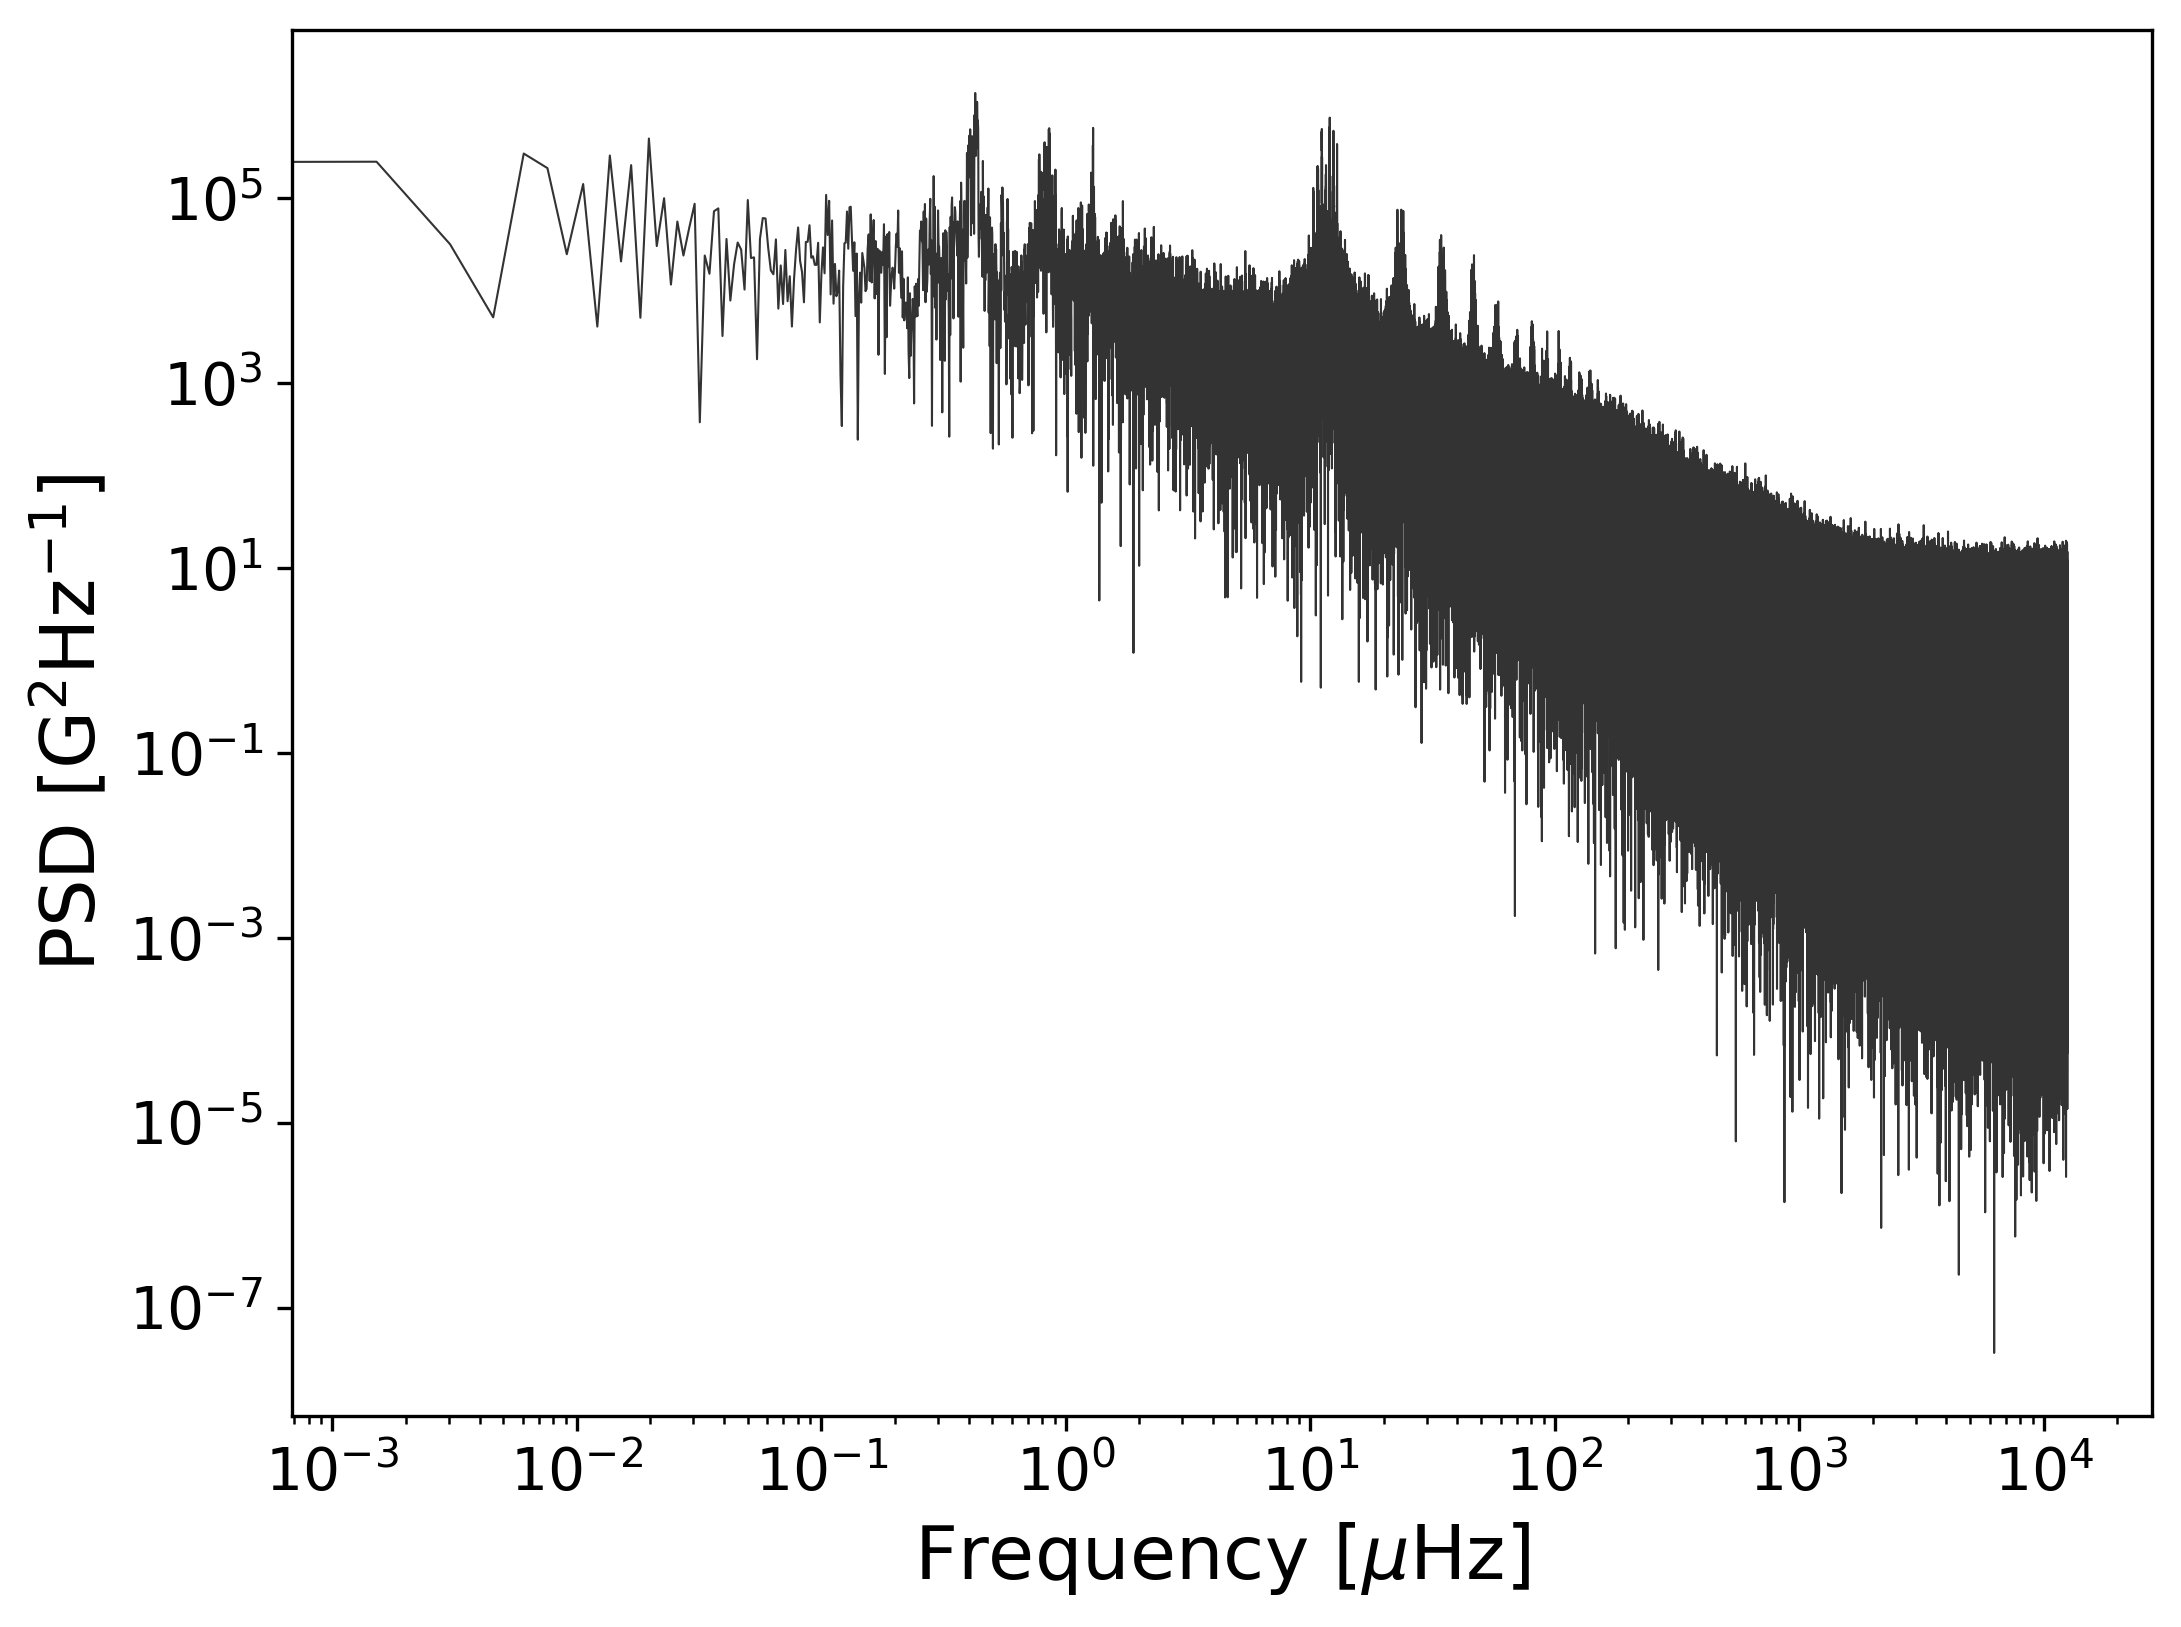
\includegraphics[width=\columnwidth]{BiSON_SMMF_FT_full.png}
	\caption{Full power spectrum of the BiSON SMMF on a logarithmic scale up to the Nyquist frequency.}
	\label{fig:BiSON_FT_full}
\end{figure}

There are a number of features in the power spectrum. First, the peaks between 0.1 -- 2.0 $\mu\mathrm{Hz}$ are a manifestation of a persistent rotational signal the SMMF. The distinct set of peaks indicates the existence of a long-lived, inhomogeneous, rotationally-modulated (RM) source. The SMMF signal exhibits a quasi-coherent nature in the time domain, and based on the comparatively short timescales for the emergence of magnetic features compared to their slow decay \citep{zwaan_solar_1981, harvey_properties_1993, hathaway_sunspot_2008}, we assume the evolution of the RM component with time is a sudden appearance and a long, exponential decay.

As we have 40-second cadence observations of the SMMF, we were able to investigate the power spectrum up to a high Nyquist frequency. This was critical to uncovering a red-noise-like component in the power spectrum. This component could arise from continuously evolving, short-lived regions of magnetic field linked to magneto-convection, akin to a random walk, which we will dub the stochastic background (SB) component. Analogous to the SB is the granulation signal observed in the Doppler-velocity measurements of the solar surface \citep{basu_asteroseismic_2017}. 

In addition, at low-frequency, there is power associated instrumental noise and activity. At very-high frequency shot-noise is captured and sets the lower limit in power in the spectrum. 

There are also side-band features in the power spectrum at multiples of $1/\mathrm{day} \sim 11.57 \, \mu\mathrm{Hz}$. The side-bands are a well-known phenomena in ground-based helioseismology. They arise from gaps in the data which are a consequence of making single-site, ground-based observations of the Sun.

The duty cycle of observations is very low, at around 15\%, therefore it is also important to take into consideration the effect that gaps in the data have on the power spectrum. Gaps in the data cause an aliasing of power from actual signal frequencies spread to other frequencies in the spectrum, and the nature of the aliasing depends on the properties of the window function of the observations. Hence before modelling the power spectrum the window function was well-characterised.

Understanding how the duty cycle of the observations affects the power spectrum we achieve will inform the way we parametrise the full model of the power spectrum.


%%%%%%%%%%%%%%%%%%%%%%%%%%%%%%%%%%%%%%%%%%%%%%%%%%%%%%%%%%%%%%%%%%%%%
\subsection{Parameterisation of the SMMF Power Spectrum}

In the frequency domain, each of the RM peaks models well as a Lorentzian distribution, similar to peak-bagging modes of solar oscillation \citep{handberg_bayesian_2011, davies_low-frequency_2014}, which is due to the quasi-coherent nature of the source. The exponential decay of the RM SMMF source gives width to the peaks in the power spectrum, which we can measure to infer their lifetime.

A single, symmetric Lorentzian peak can be modelled by equation~(\ref{eq:symm_lorentzian}), where $\nu$ is frequency, $A_n$ is the mode amplitude of the RM component, $\Gamma$ is the RM mode line-width, $\nu_n$ is RM mode frequency.

\begin{equation}
L_n(\nu; \Gamma, A_n, \nu_n) = \frac{2{A_n}^2}{\pi \Gamma} \left(1 + \left(\frac{\nu - \nu_{n}}{\Gamma /2}\right)^2\right)^{-1} 
\label{eq:symm_lorentzian}
\end{equation}

Upon closer inspection of the power specturm it is possible to see that the peak appear to exhibit an asymmetric shape, see Figure~\ref{fig:BiSON_SMMF}. Taking inspiration from \citep{howe_solar_2020}, it is possible to allow for asymmetry in the Lorentzian peak, which is controlled by the asymmetry parameter, $\alpha$, in equation~(\ref{eq:asymm_lorentzian}):

\begin{equation}
L_n(\nu; \Gamma, A_n, \nu_n) = \frac{2{A_n}^2}{\pi \Gamma(\nu)} \left(1 + \left(2X(\nu)\right)^2\right)^{-1} 
\label{eq:asymm_lorentzian}
\end{equation}

where

\begin{equation}
X(\nu) = (\nu - \nu_n)/\Gamma(\nu)
\label{eq:asymm_freq}
\end{equation}

\begin{equation}
\Gamma(\nu) = 2\Gamma / [1 + \exp^{\alpha(\nu - \nu_n)}] .
\label{eq:asymm_width}
\end{equation}

In the limit where $\alpha \rightarrow 0$, we see that the asymmetric expression equates to the symmetric expression.

The model function used to describe the RM signal in the power spectrum is given by equation~(\ref{eq:lorentzian_fit}); the sum of $N$ Lorentzian-peaks. The subscript, $n$, describes a single peak in the power spectrum; in implementing the model we constrain the mode frequencies such that they must be integer values of $\nu_0$: $\nu_n \, = \, n \nu_0$. This means that we define a single rotation frequency only, and subsequent peaks are harmonics. It is worth noting explicitly that this function assumes the line width of each Lorentzian peak is the same, only their amplitudes and central frequency differ.

When modelling the power spectrum we attempt with both the symmetric and asymmetric Lorentzian expressions, to determine whether there is a necessity for the extra parameter.

\begin{equation}
P(\nu) = \sum_{n=0}^{N} L_n(\nu; \Gamma, A_n, \nu_n)
\label{eq:lorentzian_fit}
\end{equation}


Through this formulation we can measure the lifetime of the RM component ($L$), as it is related to the line-width of the peak by equation~(\ref{eq:mode_lifetime}).

\begin{equation}
\Gamma  = (\pi L)^{-1}
\label{eq:mode_lifetime}
\end{equation}


The low-frequency power can be incorporated into the model via the inclusion of a zero-frequency centred Lorentzian, i.e. Harvey-function, given by equation~(\ref{eq:harvey}); where $\sigma$ is the characteristic amplitude of the low frequency signal, and $\tau$ describes the characteristic timescale of the excursions around zero.

\begin{equation}
H(\nu; \sigma, \tau) = \frac{4{\sigma}^2\tau}{1 + (2\pi \nu\tau)^2}
\label{eq:harvey}
\end{equation}

The SB component can also be modelled using the Harvey-function, where $\sigma$ is the characteristic amplitude of the red-noise signal and $\tau$ is its characteristic timescale.

The high frequency power is accounted for by the inclusion of a constant offset due to shot-noise, $c$.


%%%%%%%%%%%%%%%%%%%%%%%%%%%%%%%%%%%%%%%%%%%%%%%%%%%%%%%%%%%%%%%%%%%%%
\subsection{Comparison with the WSO SMMF}

To provide comparative results on the inferences from the BiSON SMMF, we repeated the analysis on the power spectrum of the WSO SMMF...


%%%%%%%%%%%%%%%%%%%%%%%%%%%%%%%%%%%%%%%%%%%%%%%%%%%%%%%%%%%%%%%%%%%%%
%%%%%%%%%%%%%%%%%%%%%%%%%%%%%%%%%%%%%%%%%%%%%%%%%%%%%%%%%%%%%%%%%%%%%
\section{Results}\label{sec:SMMF_reults}

%%%%%%%%%%%%%%%%%%%%%%%%%%%%%%%%%%%%%%%%%%%%%%%%%%%%%%%%%%%%%%%%%%%%%
\subsection{Investigation of the Window Function}\label{sec:window_fn}


Daily gaps in the data cause some power from the RM component in the power spectrum to be aliased up to higher frequencies, specifically to harmonics of the gap frequency. In this case there are daily gaps, hence power is aliased to a frequency of 1/day $\sim$~11.57 $\mu$Hz and its harmonics.

As the mode frequency (and harmonics) of the RM component are located near zero ($\nu_0 \sim \,0.4 \, \mu\mathrm{Hz}$) there are negative and positive side-bands in the complete power spectrum, however we are usually only interested in positive frequencies. When considering the aliased power, both the positive and negative side-bands must be taken into account. The aliased power is therefore located at frequencies defined in equation~(\ref{eq:sidebands}), where $i$ denotes the side-band number, and $n$ denotes the harmonic of the mode. The locations of side-bands are shown clearly to obey equation~(\ref{eq:sidebands}) in the SMMF power spectrum show in Fig.~\ref{fig:sideband_locations}.

\begin{figure}[ht!]
	\centering
	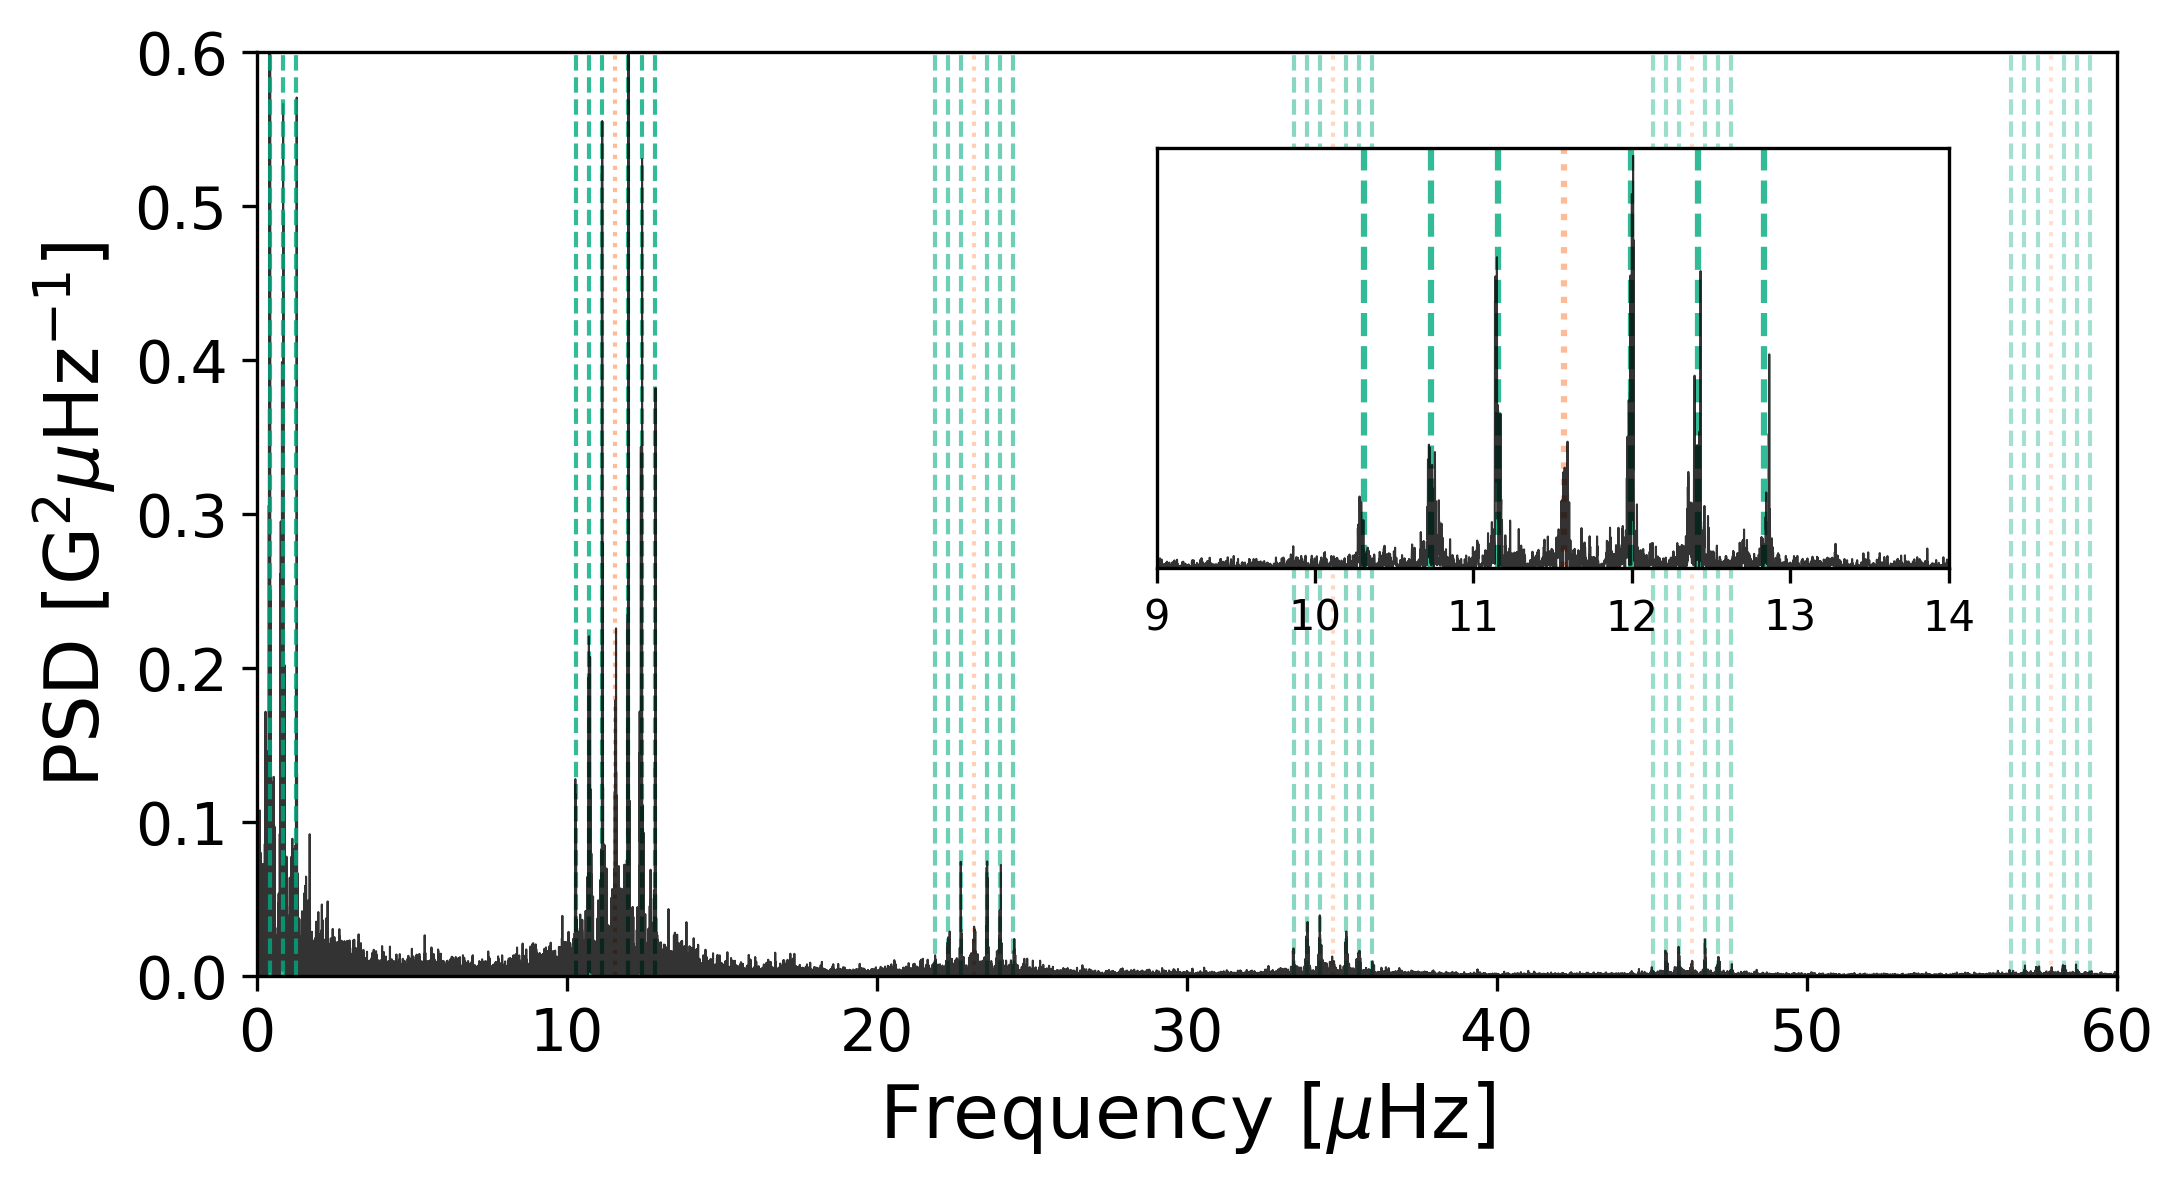
\includegraphics[width=\columnwidth]{sideband.png}
	\caption{Locations of aliased power in side-band peaks. The orange dotted-lines show the locations of frequencies at multiples of 1/day. The green dashed-lines show the location of the side-band peaks -- harmonic frequencies reflected around multiples of 1/day.  The inset shows a zoom of one set of side-band peaks around 1/day.}
	\label{fig:sideband_locations}
\end{figure}

\begin{equation}
\nu_{n, i} = i \, (\frac{1}{\mathrm{day}} \pm \nu_{n})
\label{eq:sidebands}
\end{equation}

It is clear that we could therefore use the predicted locations of the aliased power and incorporate this into the model for the full power spectrum. This would however require us to explicitly model $\sim 1100$ groups of side-bands in order to cover this effect over the entire frequency range, and each group would require a unique parameter to control the fraction of power that is contributed to the full PSD. It can become computationally expensive to model each aliased peak and there is certainly room for degeneracy issues to occur.

An alternative approach is to utilise the power spectrum of the window function itself. To do this the Fourier transform of the window function describing the duty cycle of observations was computed (i.e. $\left|\mathcal{F}\left[g(t)\right]\right|^2$), where the duty cycle function, $g(t)$, is given by equation~(\ref{eq:window}).

\begin{equation}
g(t) = 
\begin{cases} 
1 & \text{for } |B(t)| > 0 \\
0       & \text{for } |B(t)| = 0
\end{cases}
\label{eq:window}
\end{equation}

To further investigate the effects of the window function, an artificial power spectrum was simulated with a single Lorentzian peak which followed equation~(\ref{eq:lorentzian_fit}), with parameter values. By computing the inverse Fourier transform, an artificial time-series was generated over the same epoch as the BiSON SMMF observations. We were then able to examine the effects of injecting gaps into the data which were concurrent with the BiSON SMMF gaps. 

In Figure~\ref{fig:window_function_PSDs} the power spectrum of the window function is shown, as well as the noiseless input peak, and the output power spectra of the artificial data with and without the injected gaps. The power spectrum of the BiSON SMMF data is also plotted for comparison.

\begin{figure}[ht!]
	\centering
	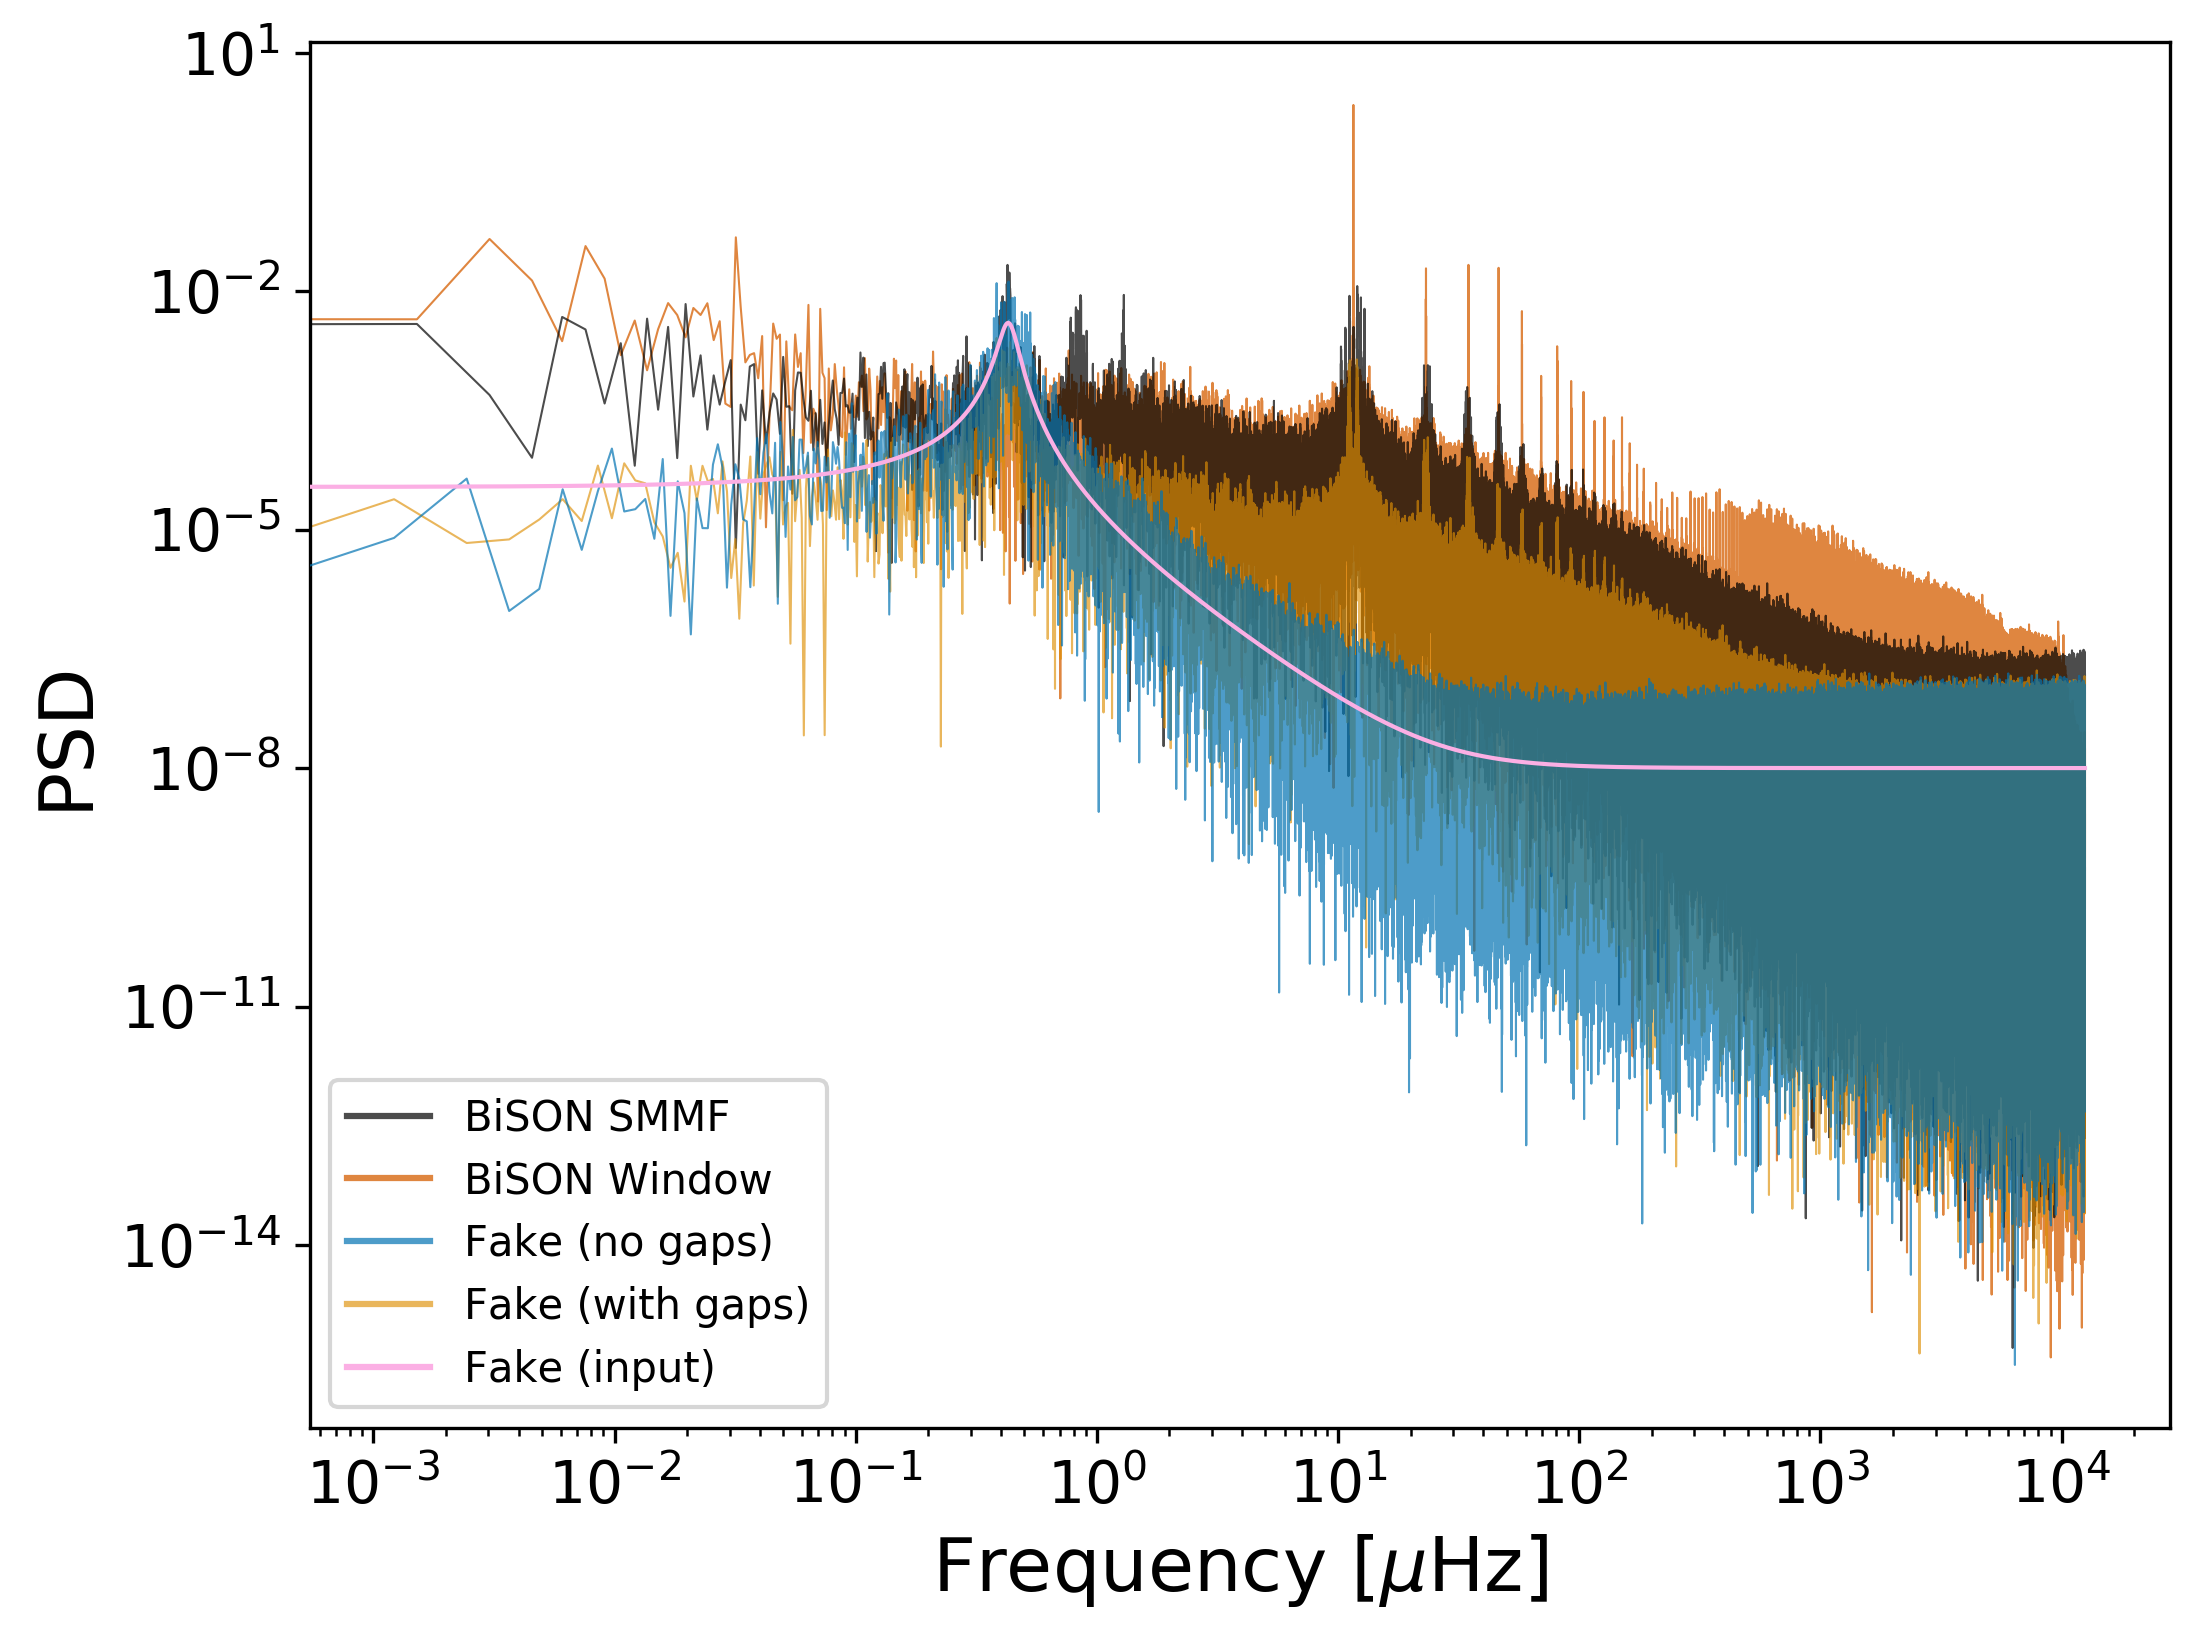
\includegraphics[width=\columnwidth]{gap_test.png}
	\caption{Shows the effects of the window function on the power spectrum. Black line: BiSON SMMF PSD; dark orange line: power spectrum of the window function; blue and light orange lines: the power spectrum of the artificial data without and with gaps, respectively; pink line: the input peak used to generate the artificial data.}
	\label{fig:window_function_PSDs}
\end{figure}

It is strikingly clear from Figure~\ref{fig:window_function_PSDs} that the shape of the spectrum of the window function has a remarkable resemblance to the BiSON SMMF spectrum and the output of the artificial spectrum with gaps injected. This shows that the periodic window function has a dominating effect on the power spectrum of the input signal which not only produces the diurnal sidebands, but also a broadband spread of the power.

Due to the broadband shape of the window function compared to the BiSON SMMF, it appears that there is actually no red-noise-like component in the SMMF and it is instead a manifestation of the gaps on the data.

We can express the  time series data ($y(t)$) as a multiplication of the signal ($f(t)$) with the window function ($g(t)$), as given by equation~(\ref{eq:timeseries}).

\begin{equation}
y(t)  = f(t) \, g(t)
\label{eq:timeseries}
\end{equation}

In the frequency domain, as the Fourier transform of a product becomes the convolution of the transformed components, it is possible to express the observed power spectrum in terms of the window function and the gap-free, model power spectrum, given in equation~(\ref{eq:PSD_fit_conv})

\begin{equation}
P'(\nu; \,{\bf a}) \, = \, P(\nu; \,{\bf a}) * \left|\mathcal{F}\left[g(t)\right]\right|^2
\label{eq:PSD_fit_conv}
\end{equation}

Therefore to model the observed power spectrum in a robust manner, which takes into account the intricacies caused by gaps in the data, we use a model which is formed of a model power spectrum, $P(\nu; \,{\bf a})$, convolved with the Fourier transform of the window function describing the duty cycle of observations (i.e. $\left|\mathcal{F}\left[g(t)\right]\right|^2$), i.e. equation~(\ref{eq:PSD_fit_conv}), where


\begin{equation}
P(\nu; \,{\bf a}) = \sum_{n=0}^{N} L_n(\nu; \Gamma, A_n, \nu_n) \, + \, H(\nu; \sigma, \tau) \, + \, c \, .
\label{eq:PSD_model}
\end{equation}

Care was taken to ensure Parseval's theorem was obeyed, and no power was lost or gained from the convolution operation. The likelihood of the resulting model from the convolution, $P'(\nu; \,{\bf a})$, was then maximised to give the best fitting parameters.





%%%%%%%%%%%%%%%%%%%%%%%%%%%%%%%%%%%%%%%%%%%%%%%%%%%%%%%%%%%%%%%%%%%%%
\subsection{BiSON Results}\label{sec:BiSON_reults}

As there were many data points in the power spectrum, each likelihood computation was computationally expensive. In order to reduce the required computation, the power spectrum was mean re-binned by a factor of 3. As the power spectrum contained independent frequency bins, the $\chi^2$ 2-D.O.F likelihood function was used and we normalised the uncertainty in the model parameters from the posterior distributions, by dividing them by $\sqrt{3}$ \citep{appourchaux_maximum_2003}. 

This likelihood evaluation doesn't fully take into account the correlated noise due to the convolution, however again due to the large quantity of data this would have required the computation of the determinant and inversion of a very large Teoplitz matrix, which would have been too expensive to compute; hence the pragmatic approach was to ignore this correlated noise in the likelihood calculation.

The mean re-sampled BiSON power spectrum was modelled against equation~(\ref{eq:PSD_fit_conv}) (with $N = 4$ peaks) using the affine-invariant Markov Chain Monte Carlo (MCMC) sampler {\verb emcee } \citep{foreman-mackey_emcee_2013} to explore the posterior parameter space. 

The prior information on each of the parameters used during the MCMC sampling were uninformed uniform distributions (denoted by $\mathcal{U}(l, u)$ with $l$ and $u$ representing the lower and upper limits of the distribution respectively). The limits were set to cover a sensible range in parameter space, whilst limiting non-physical results or frequency aliasing.

\begin{gather*}
%
\nu_0 \, \sim \,\mathcal{U}(0.38, 0.50) \> \mu\mathrm{Hz} \\
%
\Gamma \, \sim \,\mathcal{U}(0.00, 0.11)  \> \mu\mathrm{Hz} \\
%
A_1 \, \sim \,\mathcal{U}(300, 900)  \> \mathrm{mG} \\
%
A_2 \, \sim \,\mathcal{U}(100, 500)  \> \mathrm{mG} \\
%
A_3 \, \sim \,\mathcal{U}(50, 350)  \> \mathrm{mG} \\
%
A_4 \, \sim \,\mathcal{U}(20, 150)  \> \mathrm{mG} \\
%
\sigma \, \sim \,\mathcal{U}(0.10, 1000)  \> \mathrm{mG} \\
%
\tau \, \sim \,\mathcal{U}(0.10, 200)  \> 10^6 \, \mathrm{s} \\
%
c \, \sim \,\mathcal{U}(10^{-2}, 10^{2})  \> \mathrm{G}^2 \, \mathrm{Hz}^{-1} \\
%
\alpha \, \sim \,\mathcal{U}(-500, 0)\\
\end{gather*}


In Table~\ref{tab:PSD_fit_params} the median values of marginalised posterior distributions for each of the model parameters of equation~(\ref{eq:PSD_fit_conv}) are displayed. Reported uncertainties on the parameters correspond to the $1\sigma$ ($68 \%$) credible intervals either side of the median. 


\begin{table}[ht!]
	\begin{center}
		\caption{Median values of the marginalised posterior distributions for each model parameter. Numbers in brackets denote uncertainties on the last 2 digits, and all uncertainties correspond to the $68 \%$ credible intervals either side of the median.}
		\label{tab:PSD_fit_params}
		\begin{tabular}{l c c r}
			\hline
			{Parameter} & {40-s symm.} & {40-s asymm.} & {Unit} \\
			\hline
			
			{$\nu_0$} & {0.42741$\left(_{-15}^{+15}\right)$} & {0.42761$\left(_{-15}^{+15}\right)$} & {$\mu\mathrm{Hz} $}\\
			
			{$\Gamma$} & {0.03404$\left(_{-62}^{+67}\right)$} & {0.0471$\left(_{-10}^{+11}\right)$} & {$\mu\mathrm{Hz} $} \\
			
			{$A_1$} & {422.5$\pm 1.9$} & {472.8$_{-2.8}^{+2.7}$} & {$\mathrm{mG}$} \\
			
			{$A_2$} & {296.4$\pm 2.3$} & {343.8$\pm 2.9$} & {$\mathrm{mG}$} \\
			
			{$A_3$} & {209.9$\pm 2.7$} & {247.1$\pm 3.1$} & {$\mathrm{mG}$} \\
			
			{$A_4$} & {78.9$_{-4.4}^{+4.2}$} & {101.0$_{-4.8}^{+4.7}$} &  {$\mathrm{mG}$} \\	
			
			{$\tau$} & {62.1$_{-4.1}^{+4.7}$} & {84.4$_{-6.0}^{+6.8}$} & {$\mathrm{hours}$} \\	
			
			{$\sigma$} & {200.8$\pm 3.2$} & {183.3$\pm 3.4$} &  {$\mathrm{mG}$} \\	
			
			{$bgnd$} & {1.3411$\left(_{-10}^{+10}\right)$} & {1.3399$\left(_{-10}^{+10}\right)$}  & {$\mathrm{G}^2\mathrm{Hz}^{-1}$} \\	
			
			{$\alpha$} & {--} & {-134.6$_{-5.5}^{+5.4}$} & {--} \\	
			\hline
		\end{tabular}
	\end{center}
\end{table}

As the asymmetry parameter converged reasonably within the prior bounds we therefore deduce that the extra parameter was necessary, and the model utilising asymmetric Lorentzian peaks was a better fit to the data than the model with symmetric Lorentzian peaks.

The central frequency of this model, $\nu_0$ implies a rotation period of $27.10^{+0.01}_{-0.01}$~days, and accounting for sidereal rotation, $25.23^{+0.01}_{-0.01}$~days. The rotation period measured is in agreement with other literature for the rotation signal in the SMMF \citep{chaplin_studies_2003, xie_temporal_2017}. 

According to the model for differential rotation given by \citet{snodgrass_magnetic_1983} and \citet{brown_inferring_1989}, the measured rotation period implies the RM component of the SMMF is sensitive to a time-averaged latitude of around $12^{\circ}$. This latitude is consistent with the latitudes spanned by sunspots and ARs over the solar activity cycle \citep{maunder_note_1904, mcintosh_deciphering_2014, thomas_asteroseismic_2019}, and particularly during the declining phase of the solar cycle. This strongly implies that the origin of the RM component of the SMMF is linked to active regions of magnetic field.

Furthermore, from the measured line-width of the Lorentzian peaks, we have calculated the lifetime of the RM component using equation~(\ref{eq:mode_lifetime}). The line-width suggests a RM lifetime of $78.2_{-1.7}^{+1.8}$~days, which is in the range 11~--~11.5~weeks. The typical lifetime of active magnetic regions and sunspots is usually on the order of weeks to months \citep{zwaan_solar_1981, howard_sunspot_2001, hathaway_sunspot_2008}, therefore the observations of the SMMF by BiSON measure a lifetime of the RM component which is consistent with the lifetime of ARs and sunspot, suggesting them as a possible source of the signal.


%%%%%%%%%%%%%%%%%%%%%%%%%%%%%%%%%%%%%%%%%%%%%%%%%%%%%%%%%%%%%%%%%%%%%
\subsection{WSO Results}\label{sec:WSO_reults}



%%%%%%%%%%%%%%%%%%%%%%%%%%%%%%%%%%%%%%%%%%%%%%%%%%%%%%%%%%%%%%%%%%%%%
%%%%%%%%%%%%%%%%%%%%%%%%%%%%%%%%%%%%%%%%%%%%%%%%%%%%%%%%%%%%%%%%%%%%%
\section{Simulations}\label{sec:SMMF_artificial}



%%%%%%%%%%%%%%%%%%%%%%%%%%%%%%%%%%%%%%%%%%%%%%%%%%%%%%%%%%%%%%%%%%%%%
%%%%%%%%%%%%%%%%%%%%%%%%%%%%%%%%%%%%%%%%%%%%%%%%%%%%%%%%%%%%%%%%%%%%%
\section{Investigations on the Presence of Rossby Modes}\label{sec:SMMF_rmode}





%%%%%%%%%%%%%%%%%%%%%%%%%%%%%%%%%%%%%%%%%%%%%%%%%%%%%%%%%%%%%%%%%%%%%
%%%%%%%%%%%%%%%%%%%%%%%%%%%%%%%%%%%%%%%%%%%%%%%%%%%%%%%%%%%%%%%%%%%%%
\section{Summary}\label{sec:SMMF_summary}